%!TEX TS-program = pdflatex
%!TEX root = tesi.tex
%!TEX encoding = UTF-8 Unicode

% in figura~\ref{fig:p1_overview}.
%\begin{figure}[ht]
%  \begin{center}
%    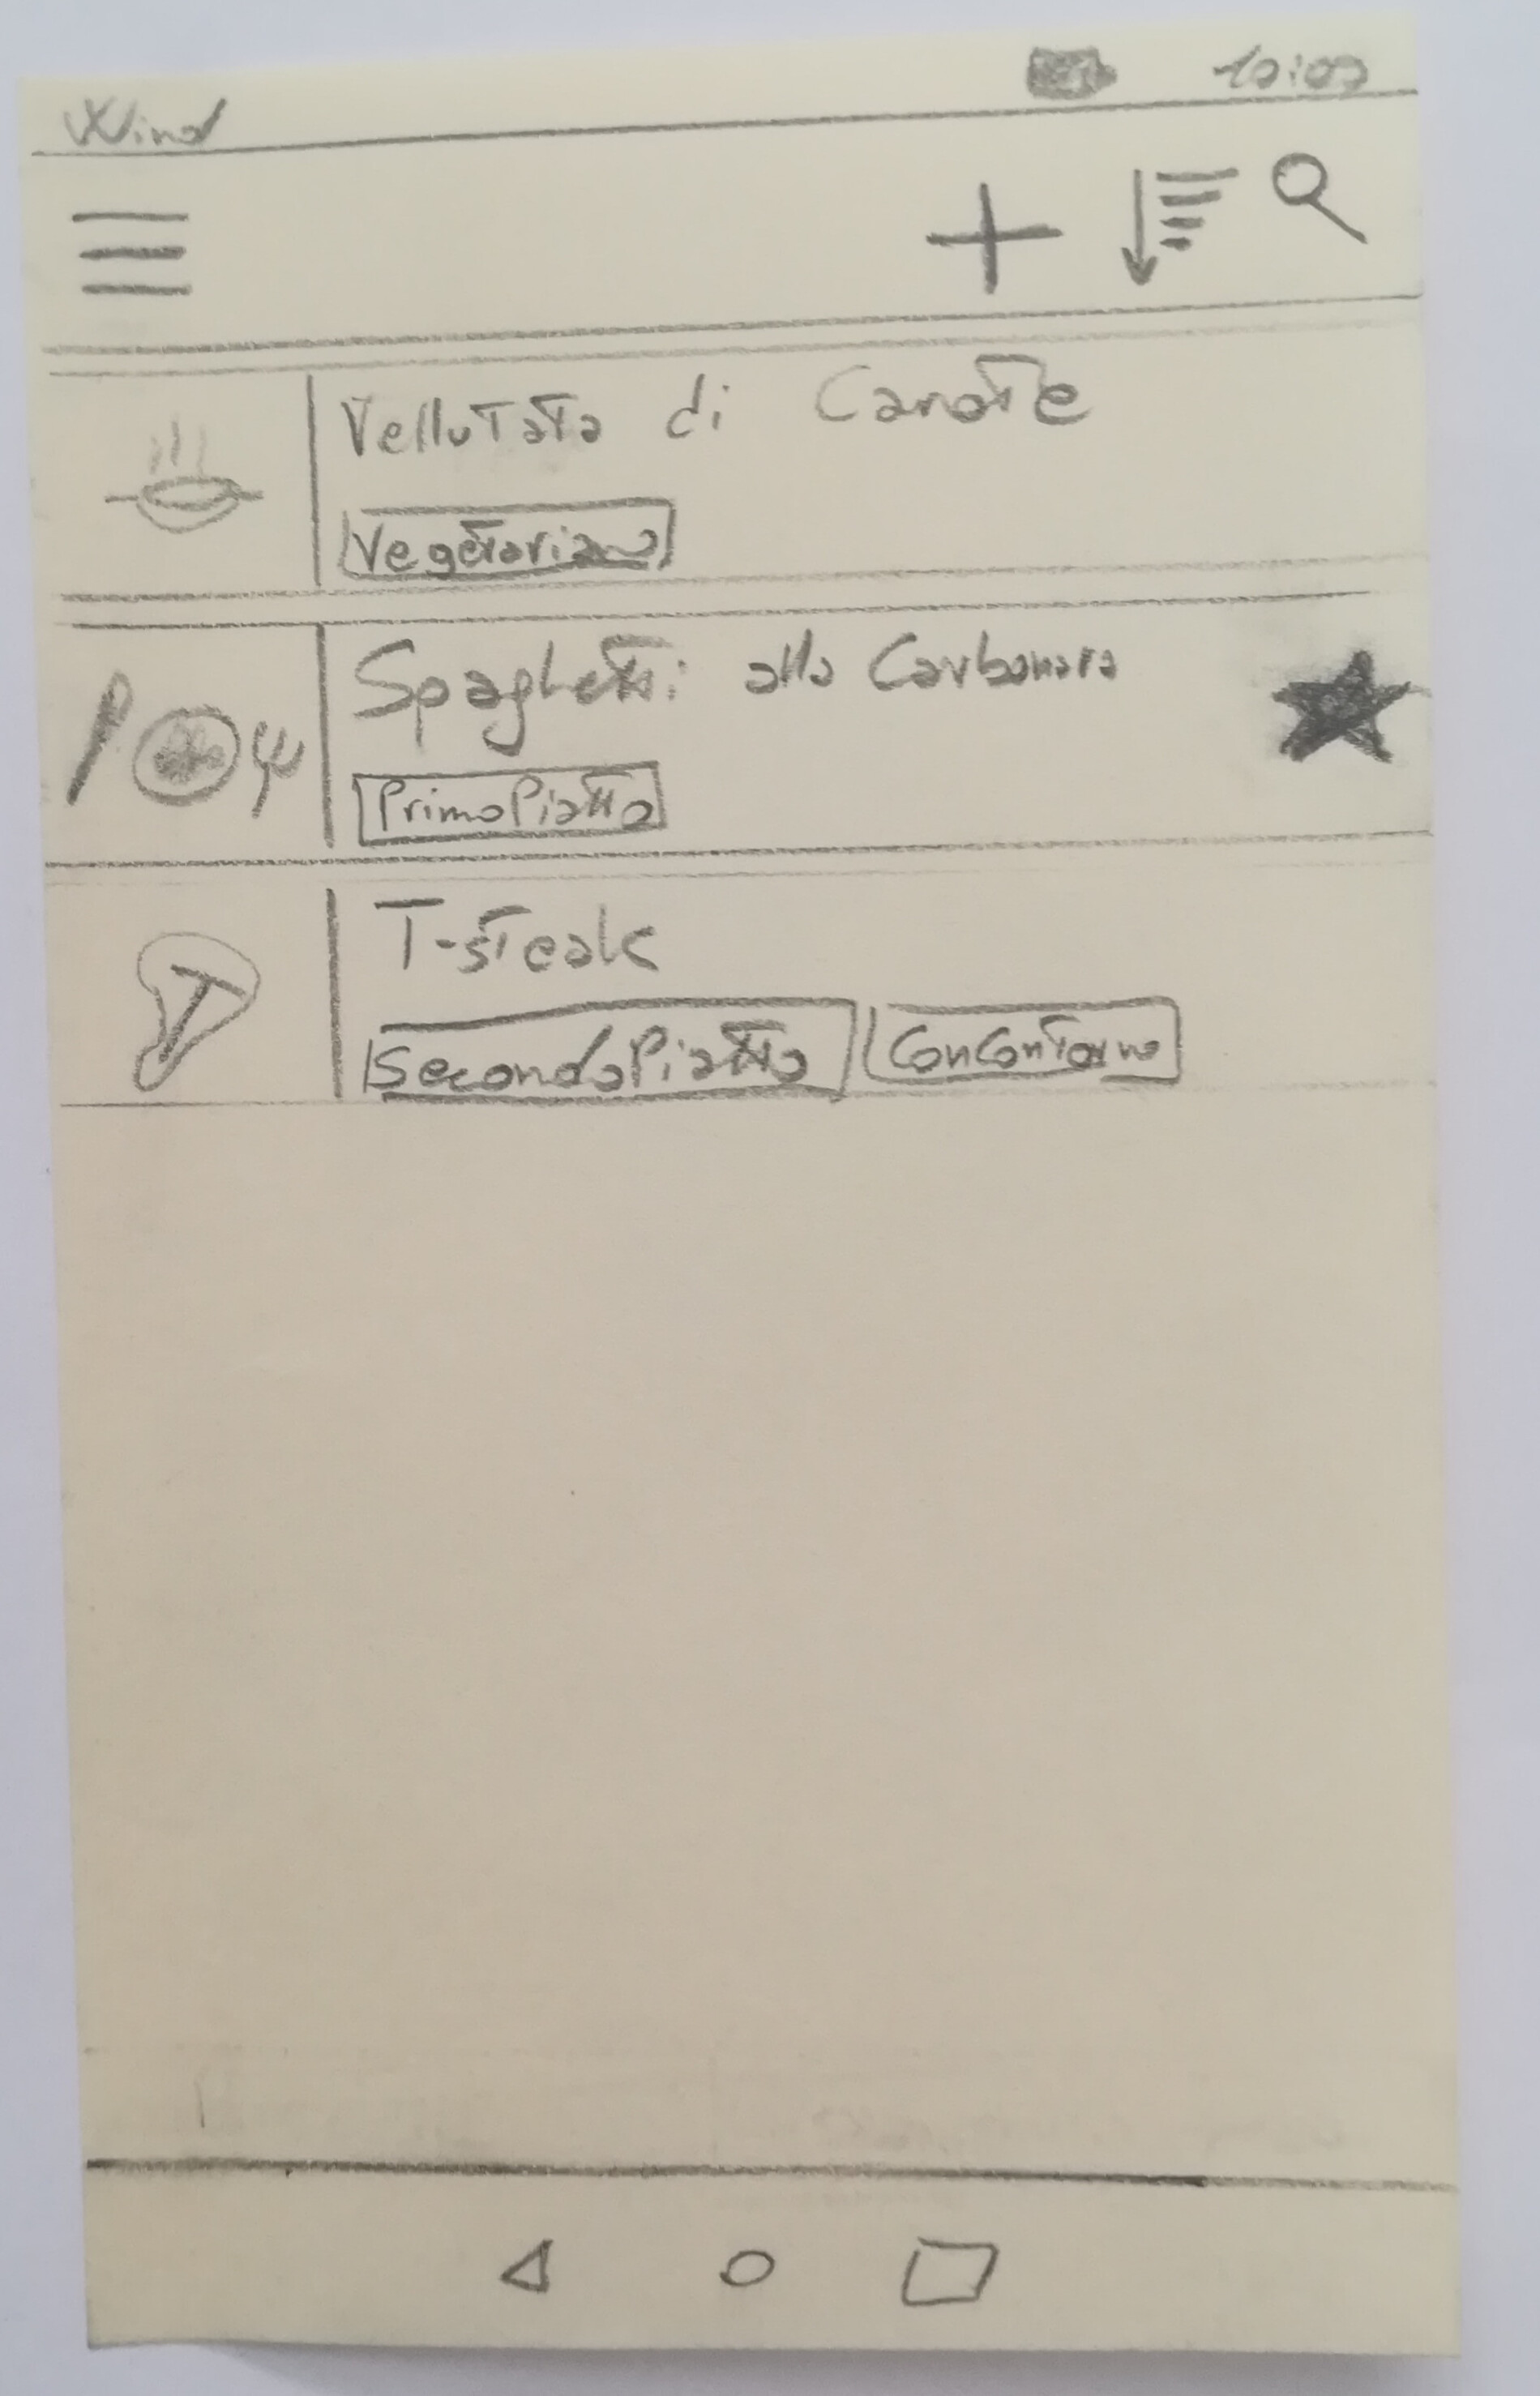
\includegraphics[width=0.6\textwidth]{prototipo1/main_ricette_lista_tags}
%    \caption{Primo storyboard}
%    \label{fig:roa}
%  \end{center}
%\end{figure}







\section{Secondo Assignment}

\subsection{Primo Prototipo Low-Fidelity}

%Il risultato di una prima prototipizzazione è riportato in figura~\ref{fig:p1_overview}.
%Come si può 
%
%\begin{figure}[ht]
%  \begin{center}
%    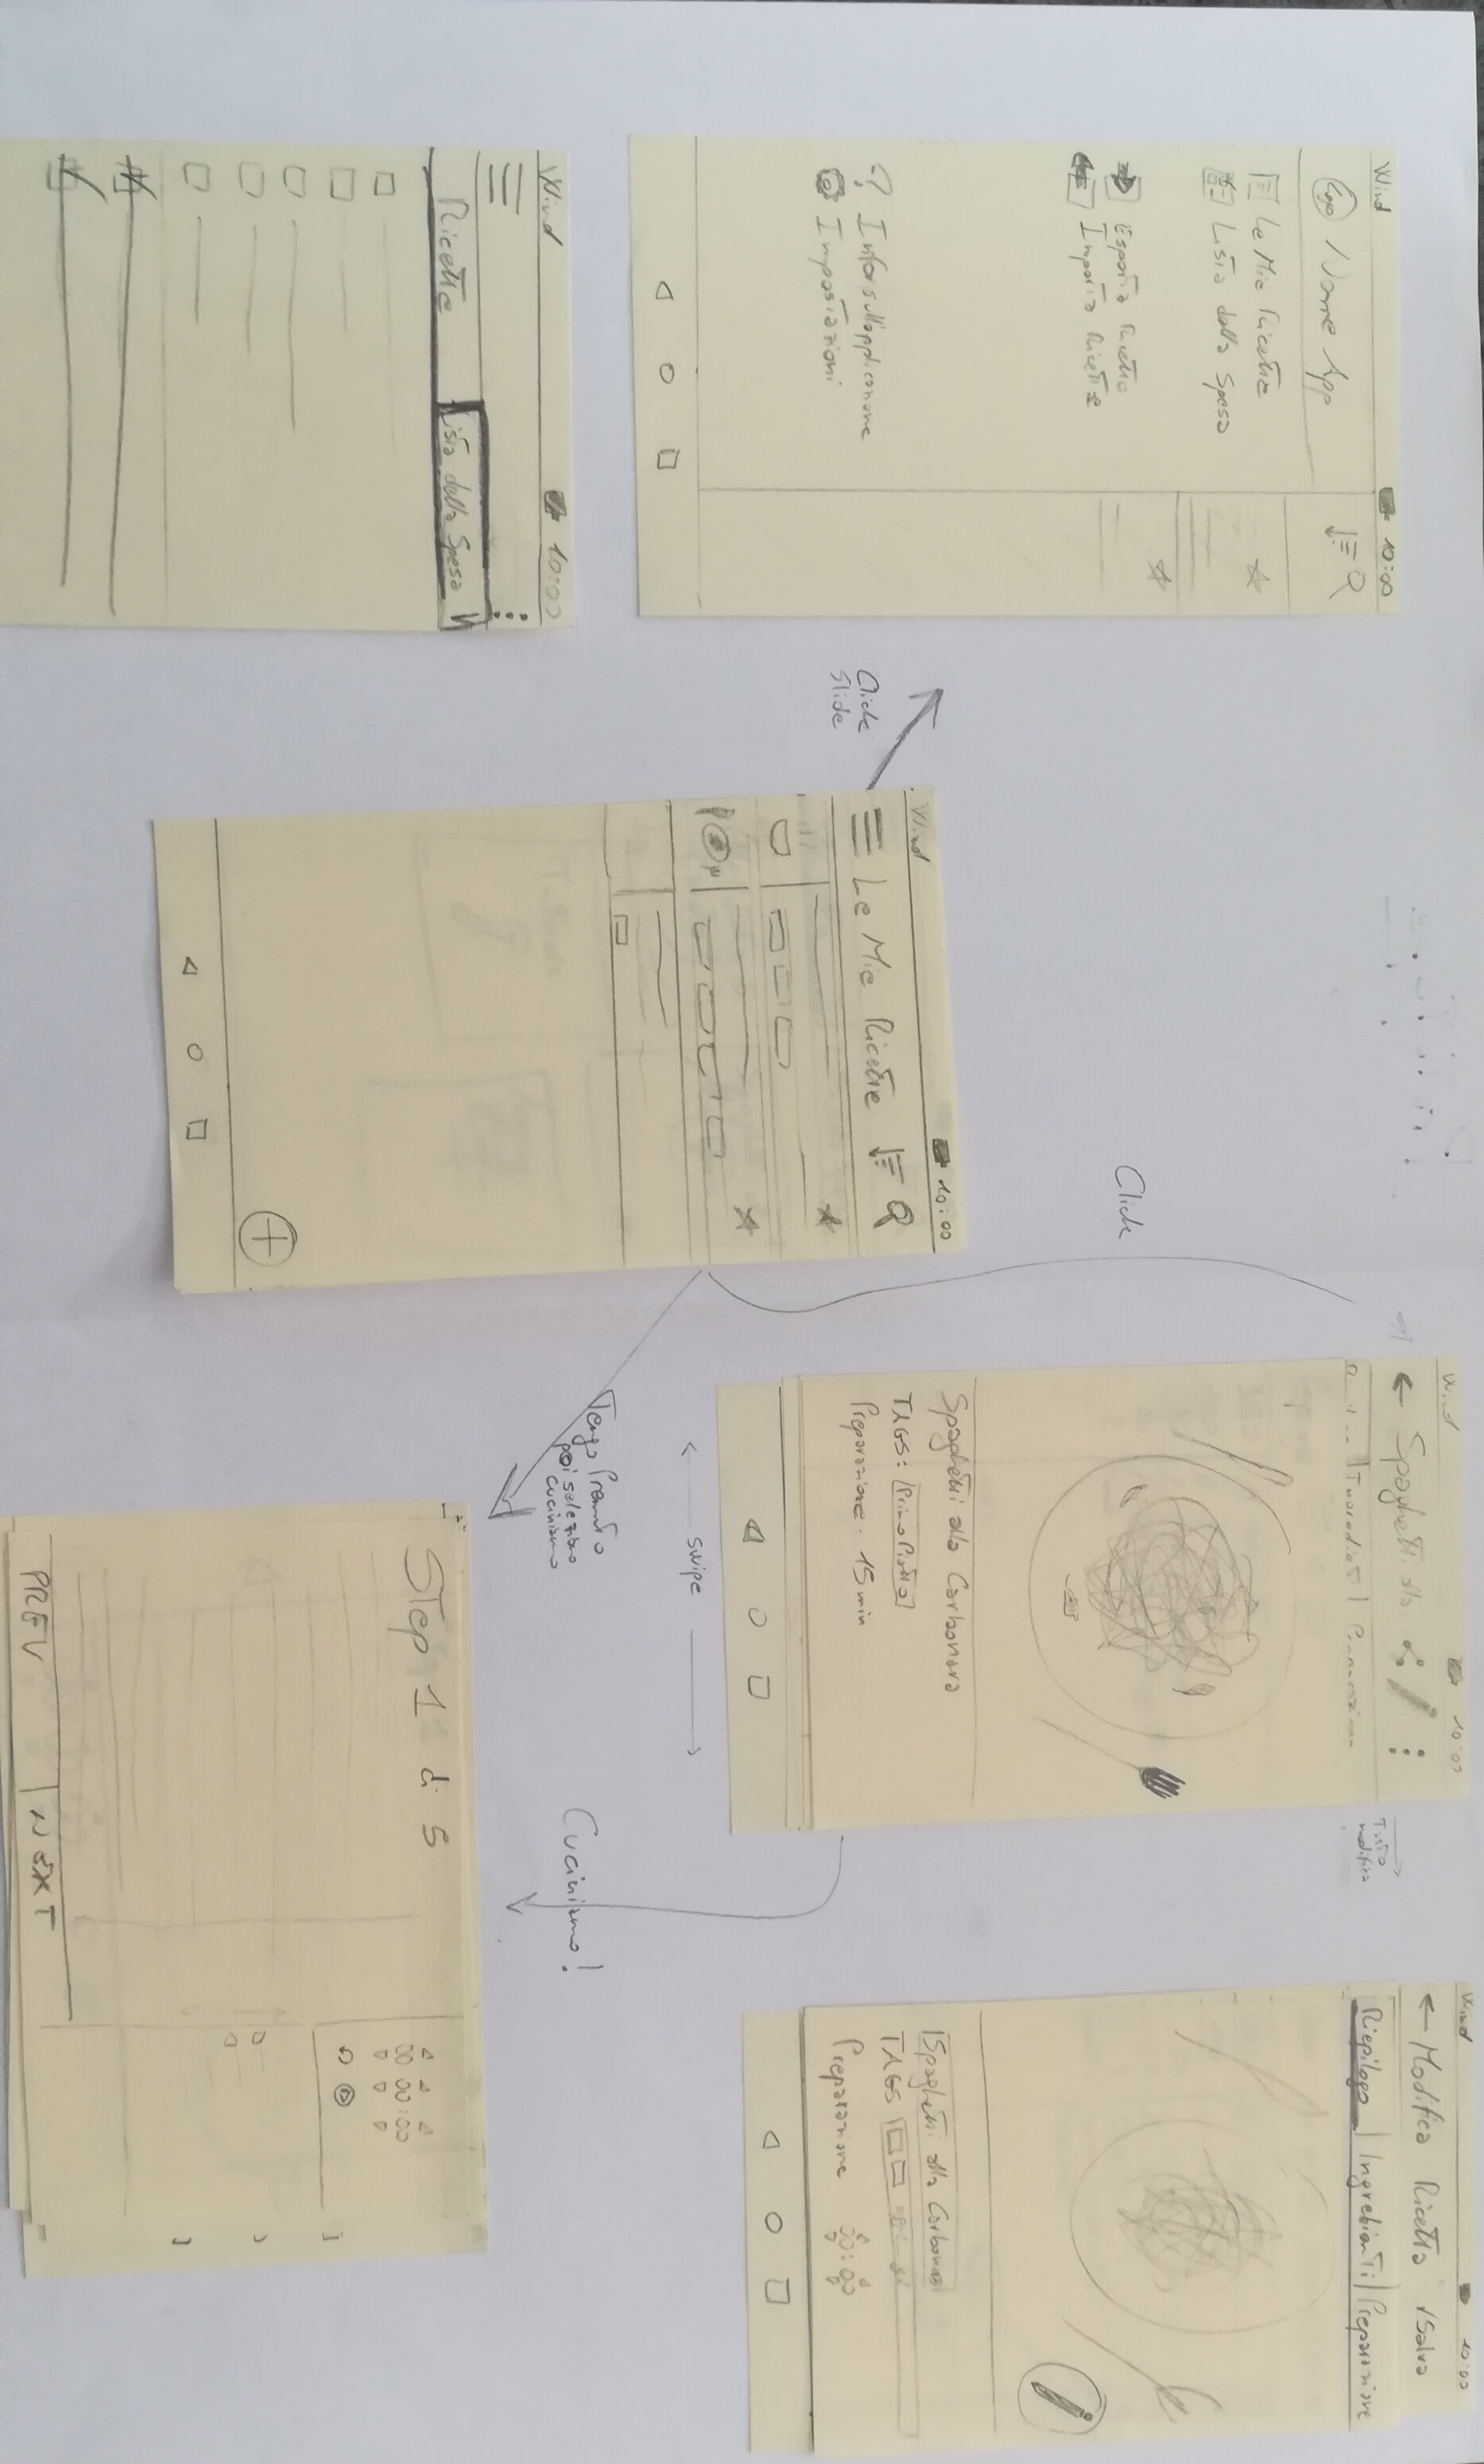
\includegraphics[width=0.6\textwidth, angle=90]{prototipo1/overview}
%    \caption{Primo storyboard}
%    \label{fig:p1_overview}
%  \end{center}
%\end{figure}

In figura~\ref{fig:p1_main} a sinistra è riportata la schermata principale dell'applicazione.
Le ricette vengono mostrate in una lista, ogni elemento mostra l'immagine associata alla ricetta, il suo titolo, eventuali etichette (ad esempio primo piatto, secondo piatto, vegetariano, contorno, \dots ) e se la ricetta appartiene ai preferiti.
I tasti in alto a sinistra indicano la possibilità di aggiungere una nuova ricetta, ordinare le ricette oppure cercarne una.
Nella schermata affianco si è valutata la possibilità di spostare il tasto di creazione di una nuova ricetta in un \textit{floating action button} posizionato in basso a destra.

\begin{figure}[ht]
  \begin{center}
    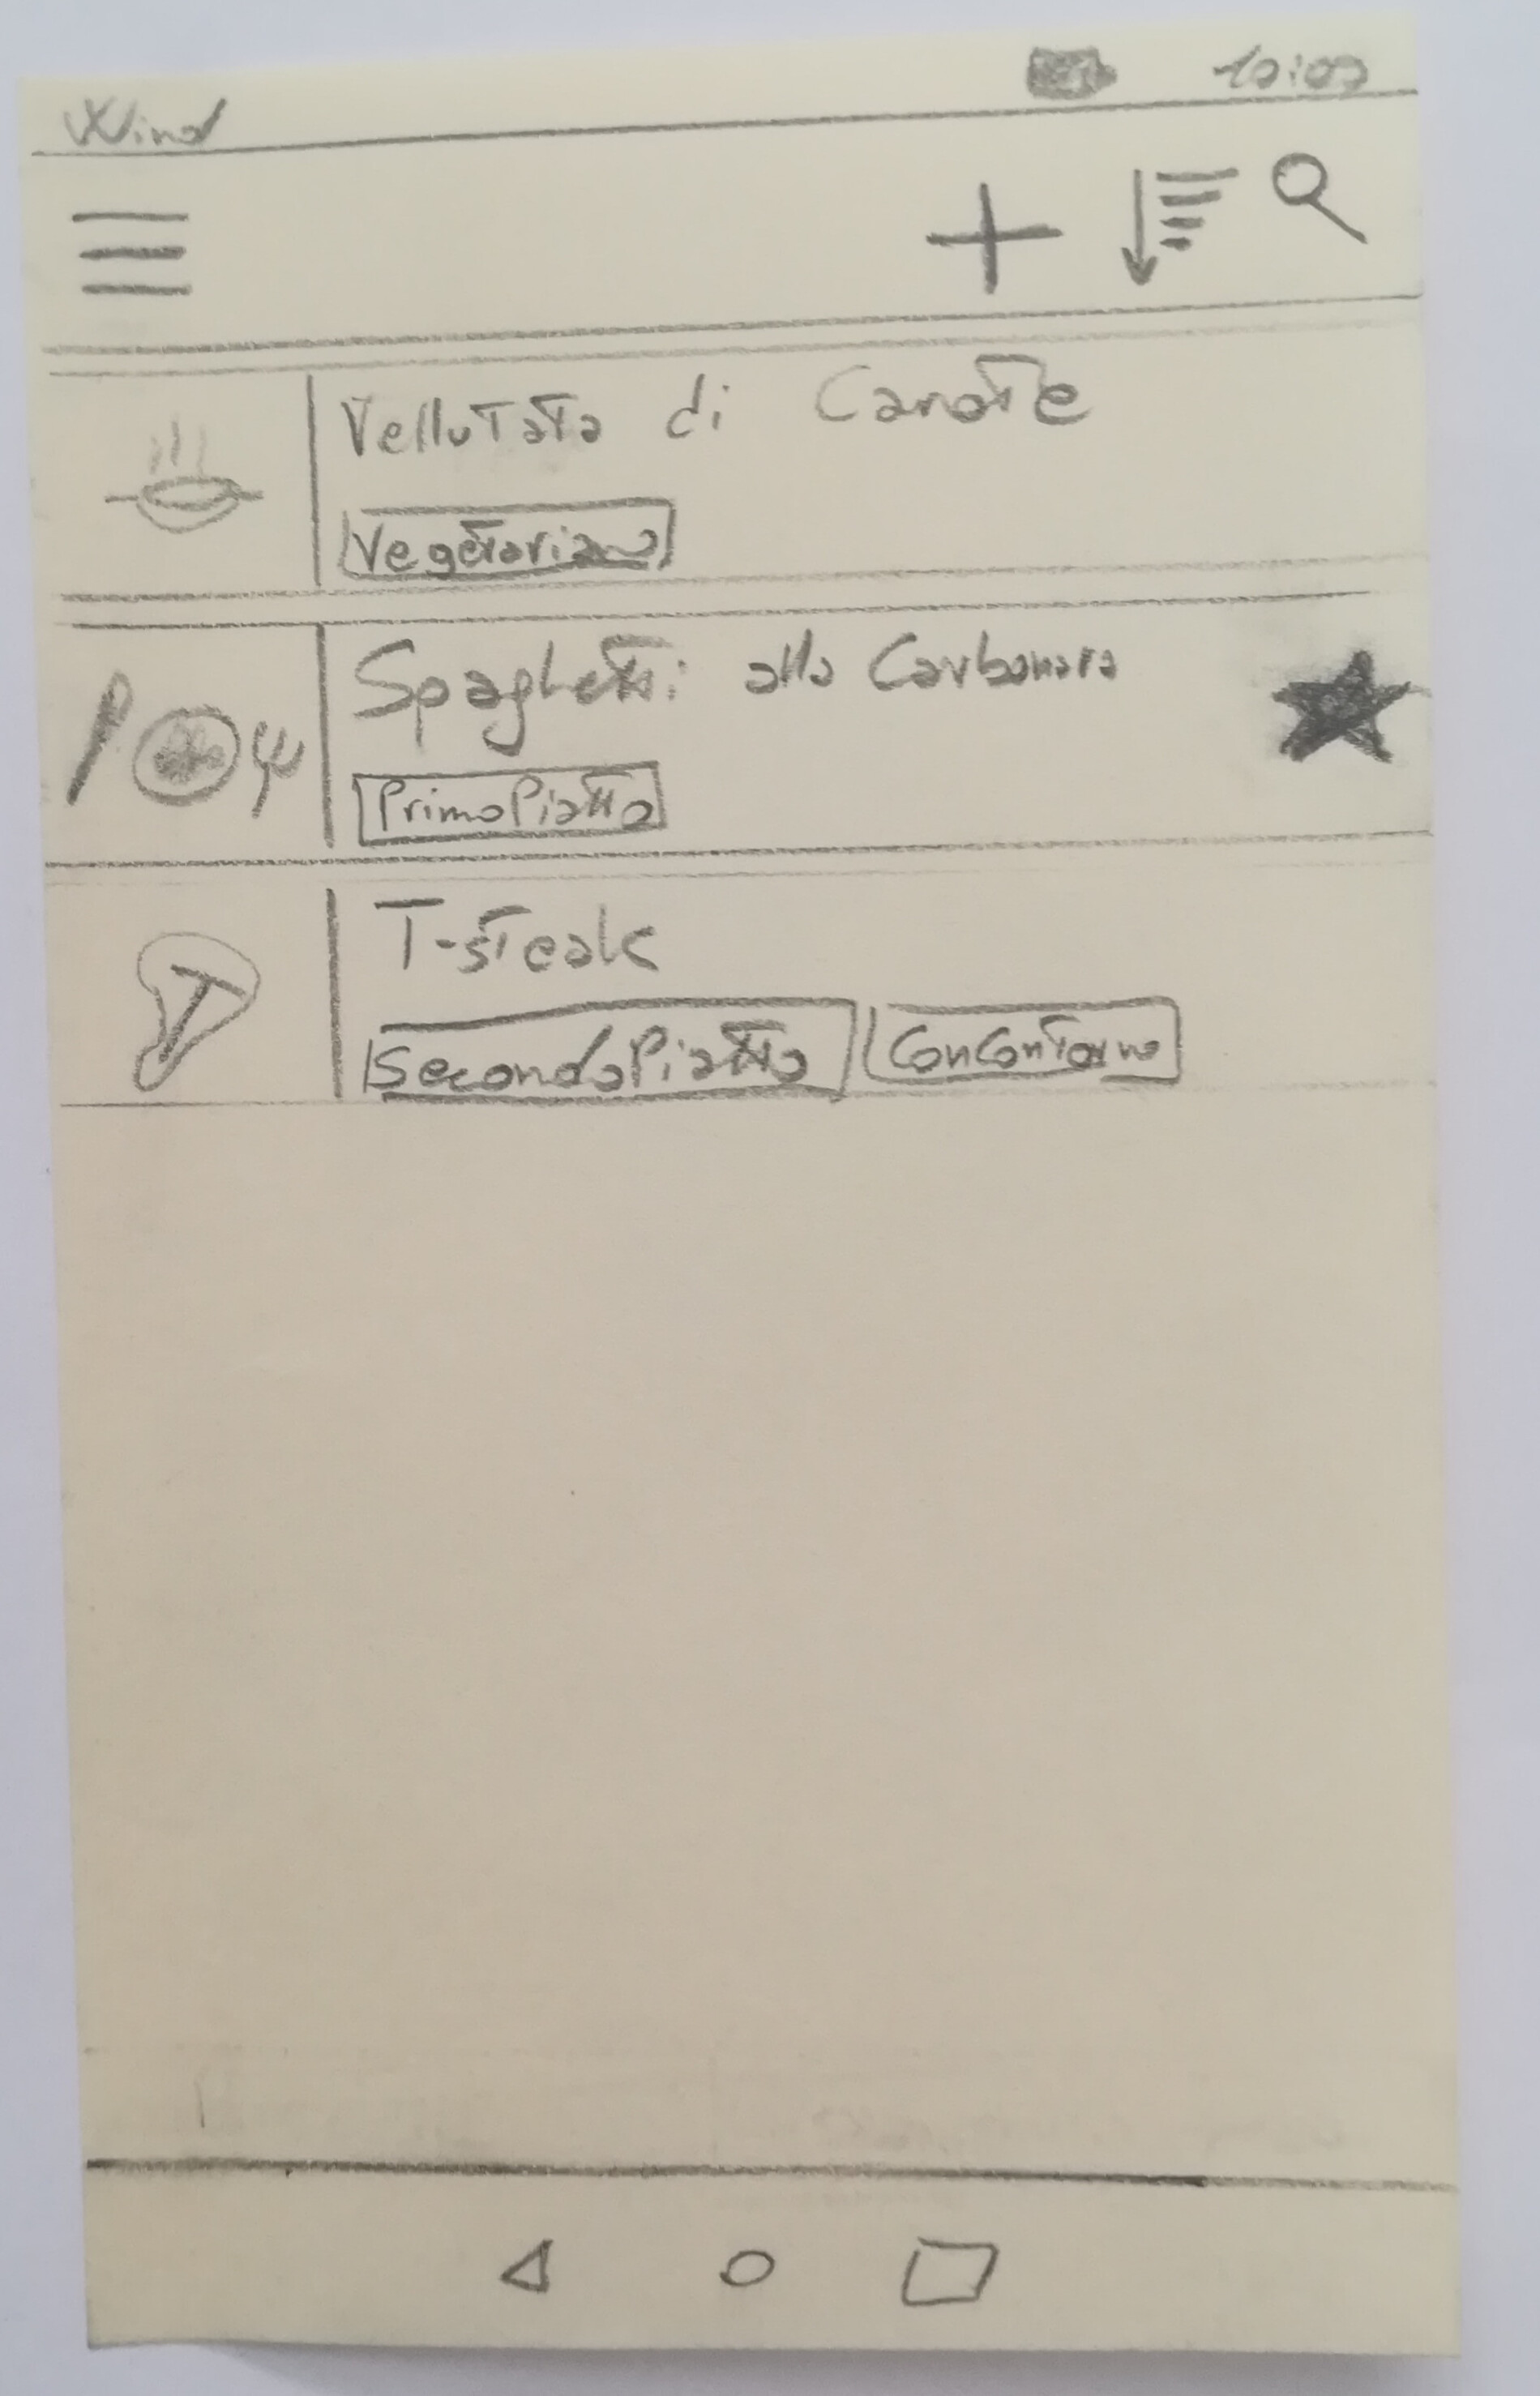
\includegraphics[width=0.45\textwidth]{prototipo1/main_ricette_lista_tags}
    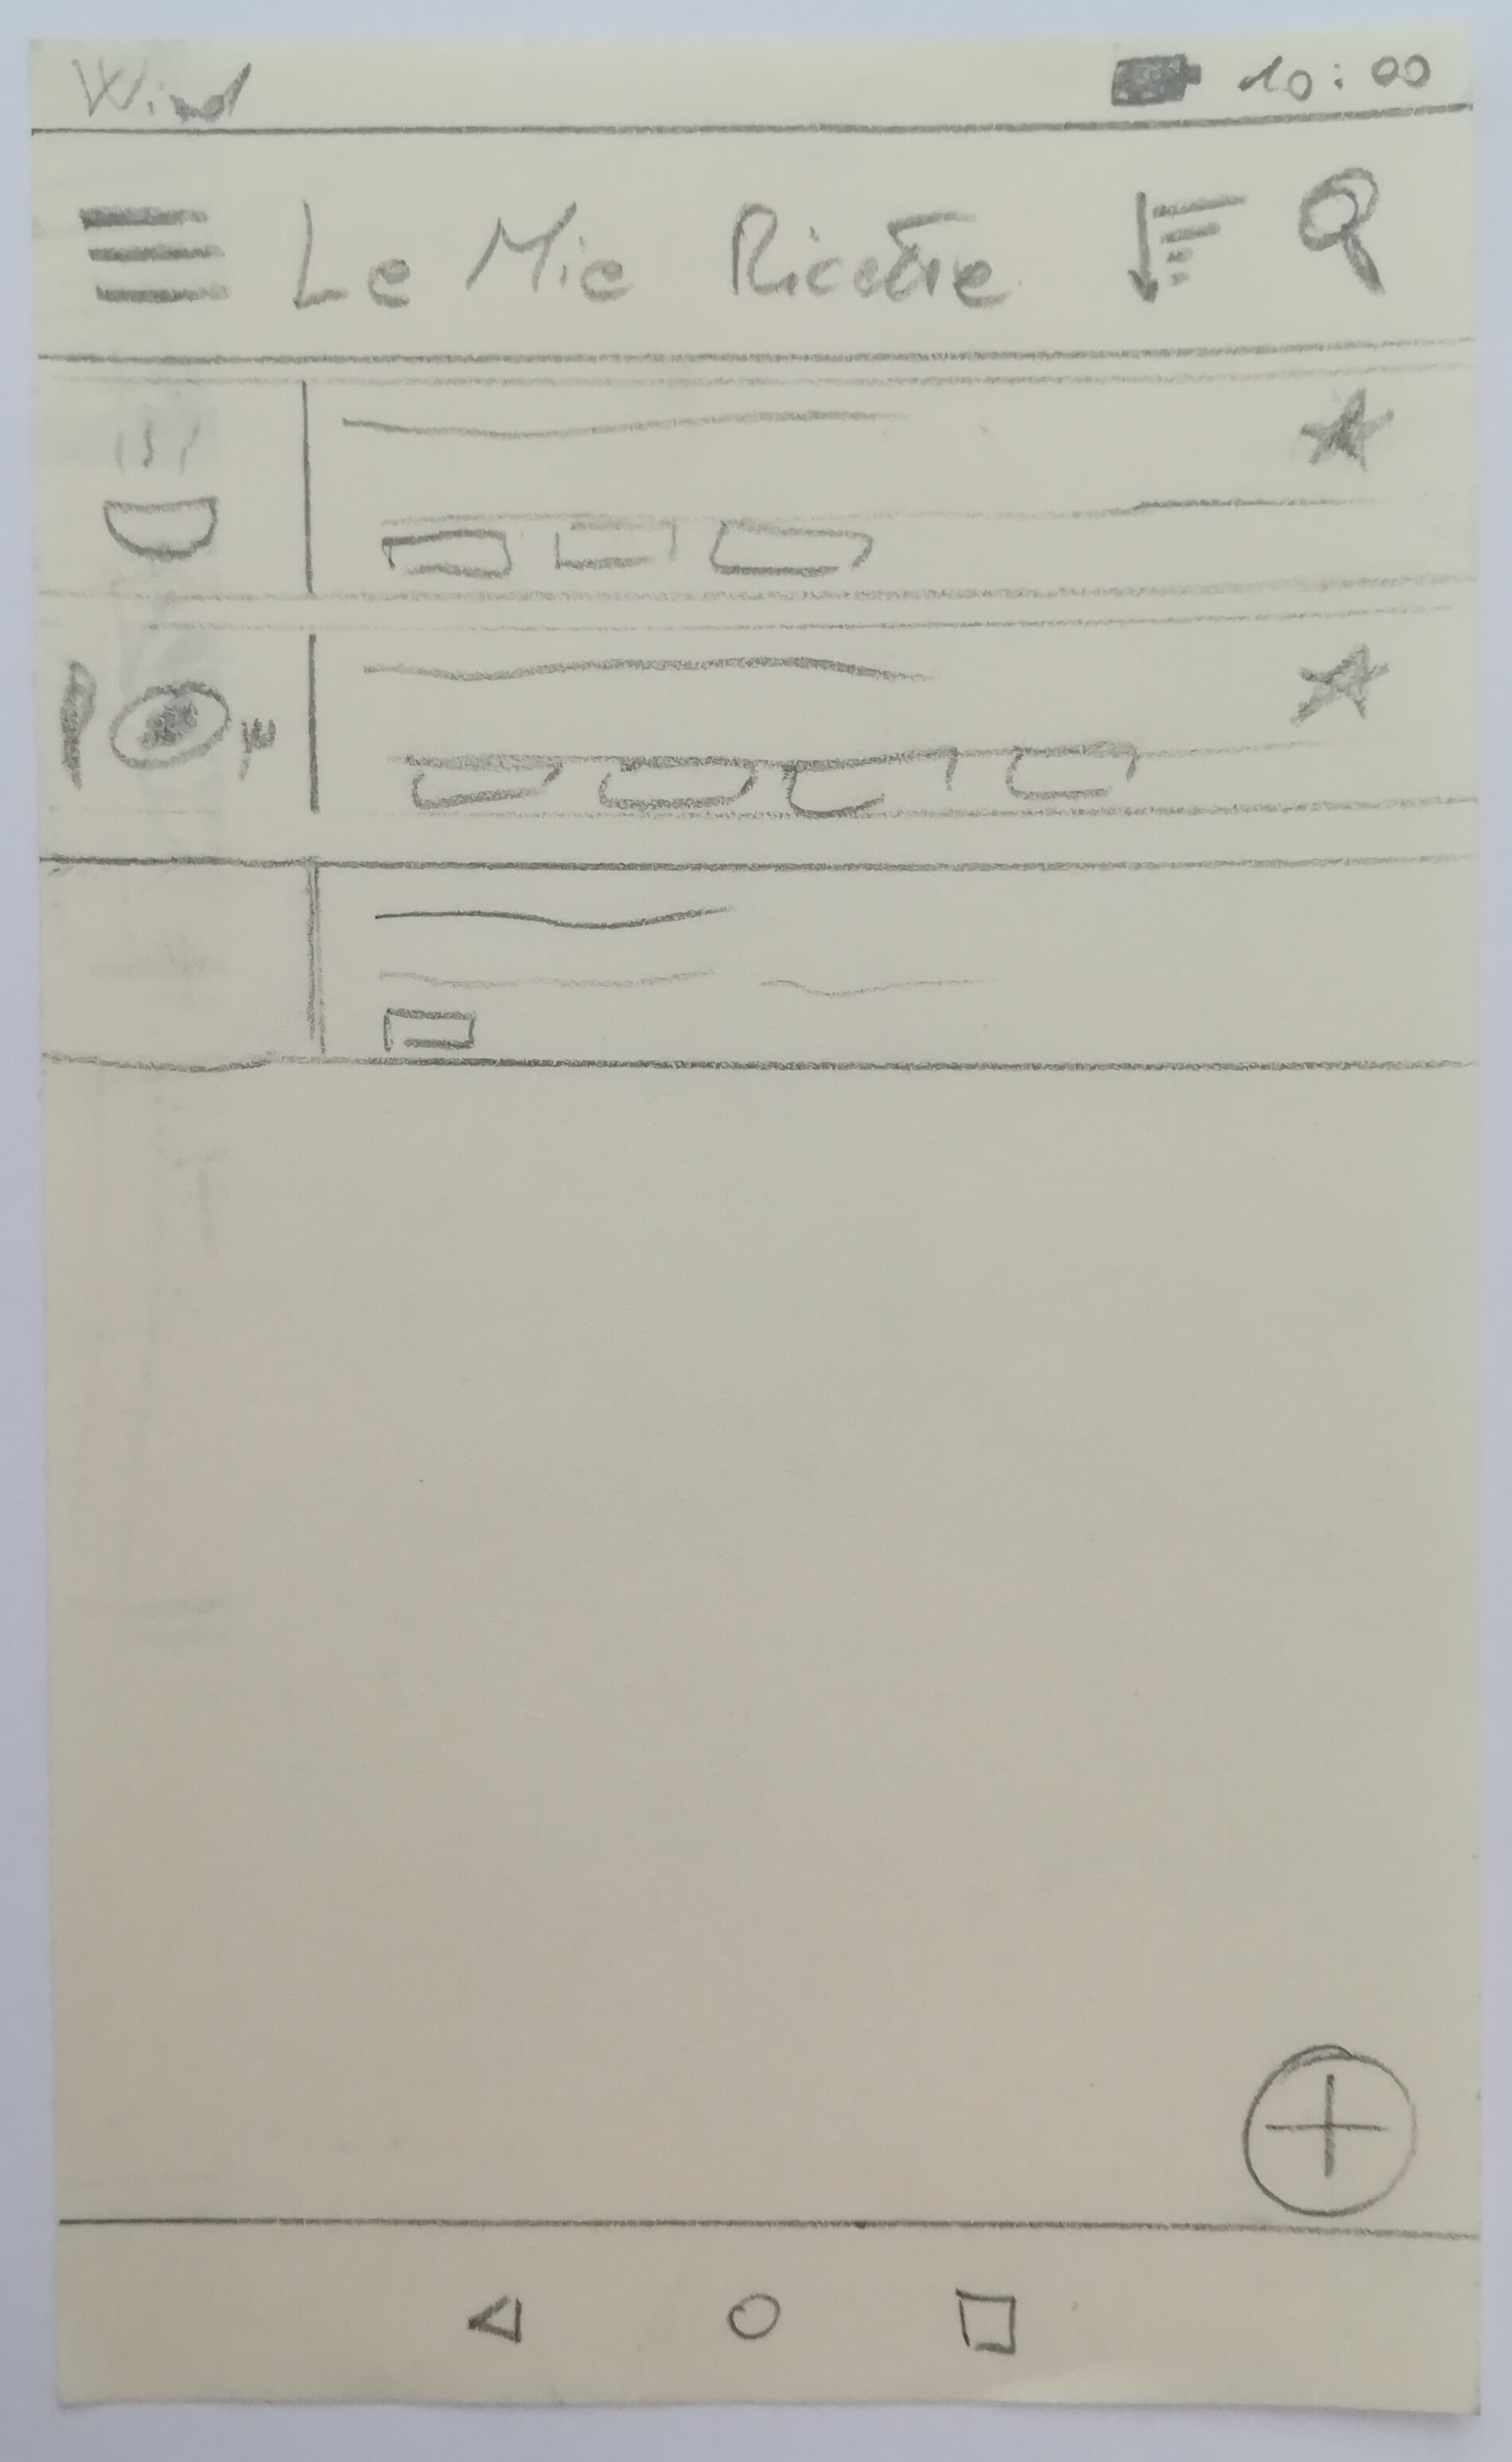
\includegraphics[width=0.43\textwidth]{prototipo1/main_ricette_lista_tags_fab}
    \caption{Schermata principale}
    \label{fig:p1_main}
  \end{center}
\end{figure}

\clearpage
Premendo il tasto in alto a sinistra si apre una TODO laterale, riportata a sinistra in figura \ref{fig:p1_lista_spesa}.
Qui è possibile effettuare varie operazioni, tra cui visualizzare la lista della spesa.
Quest'ultima è divisa in due sezioni in modo che risulti chiaro quali sono gli ingredienti ancora da comprare e quali invece sono già stati acquistati.

\begin{figure}[ht]
  \begin{center}
    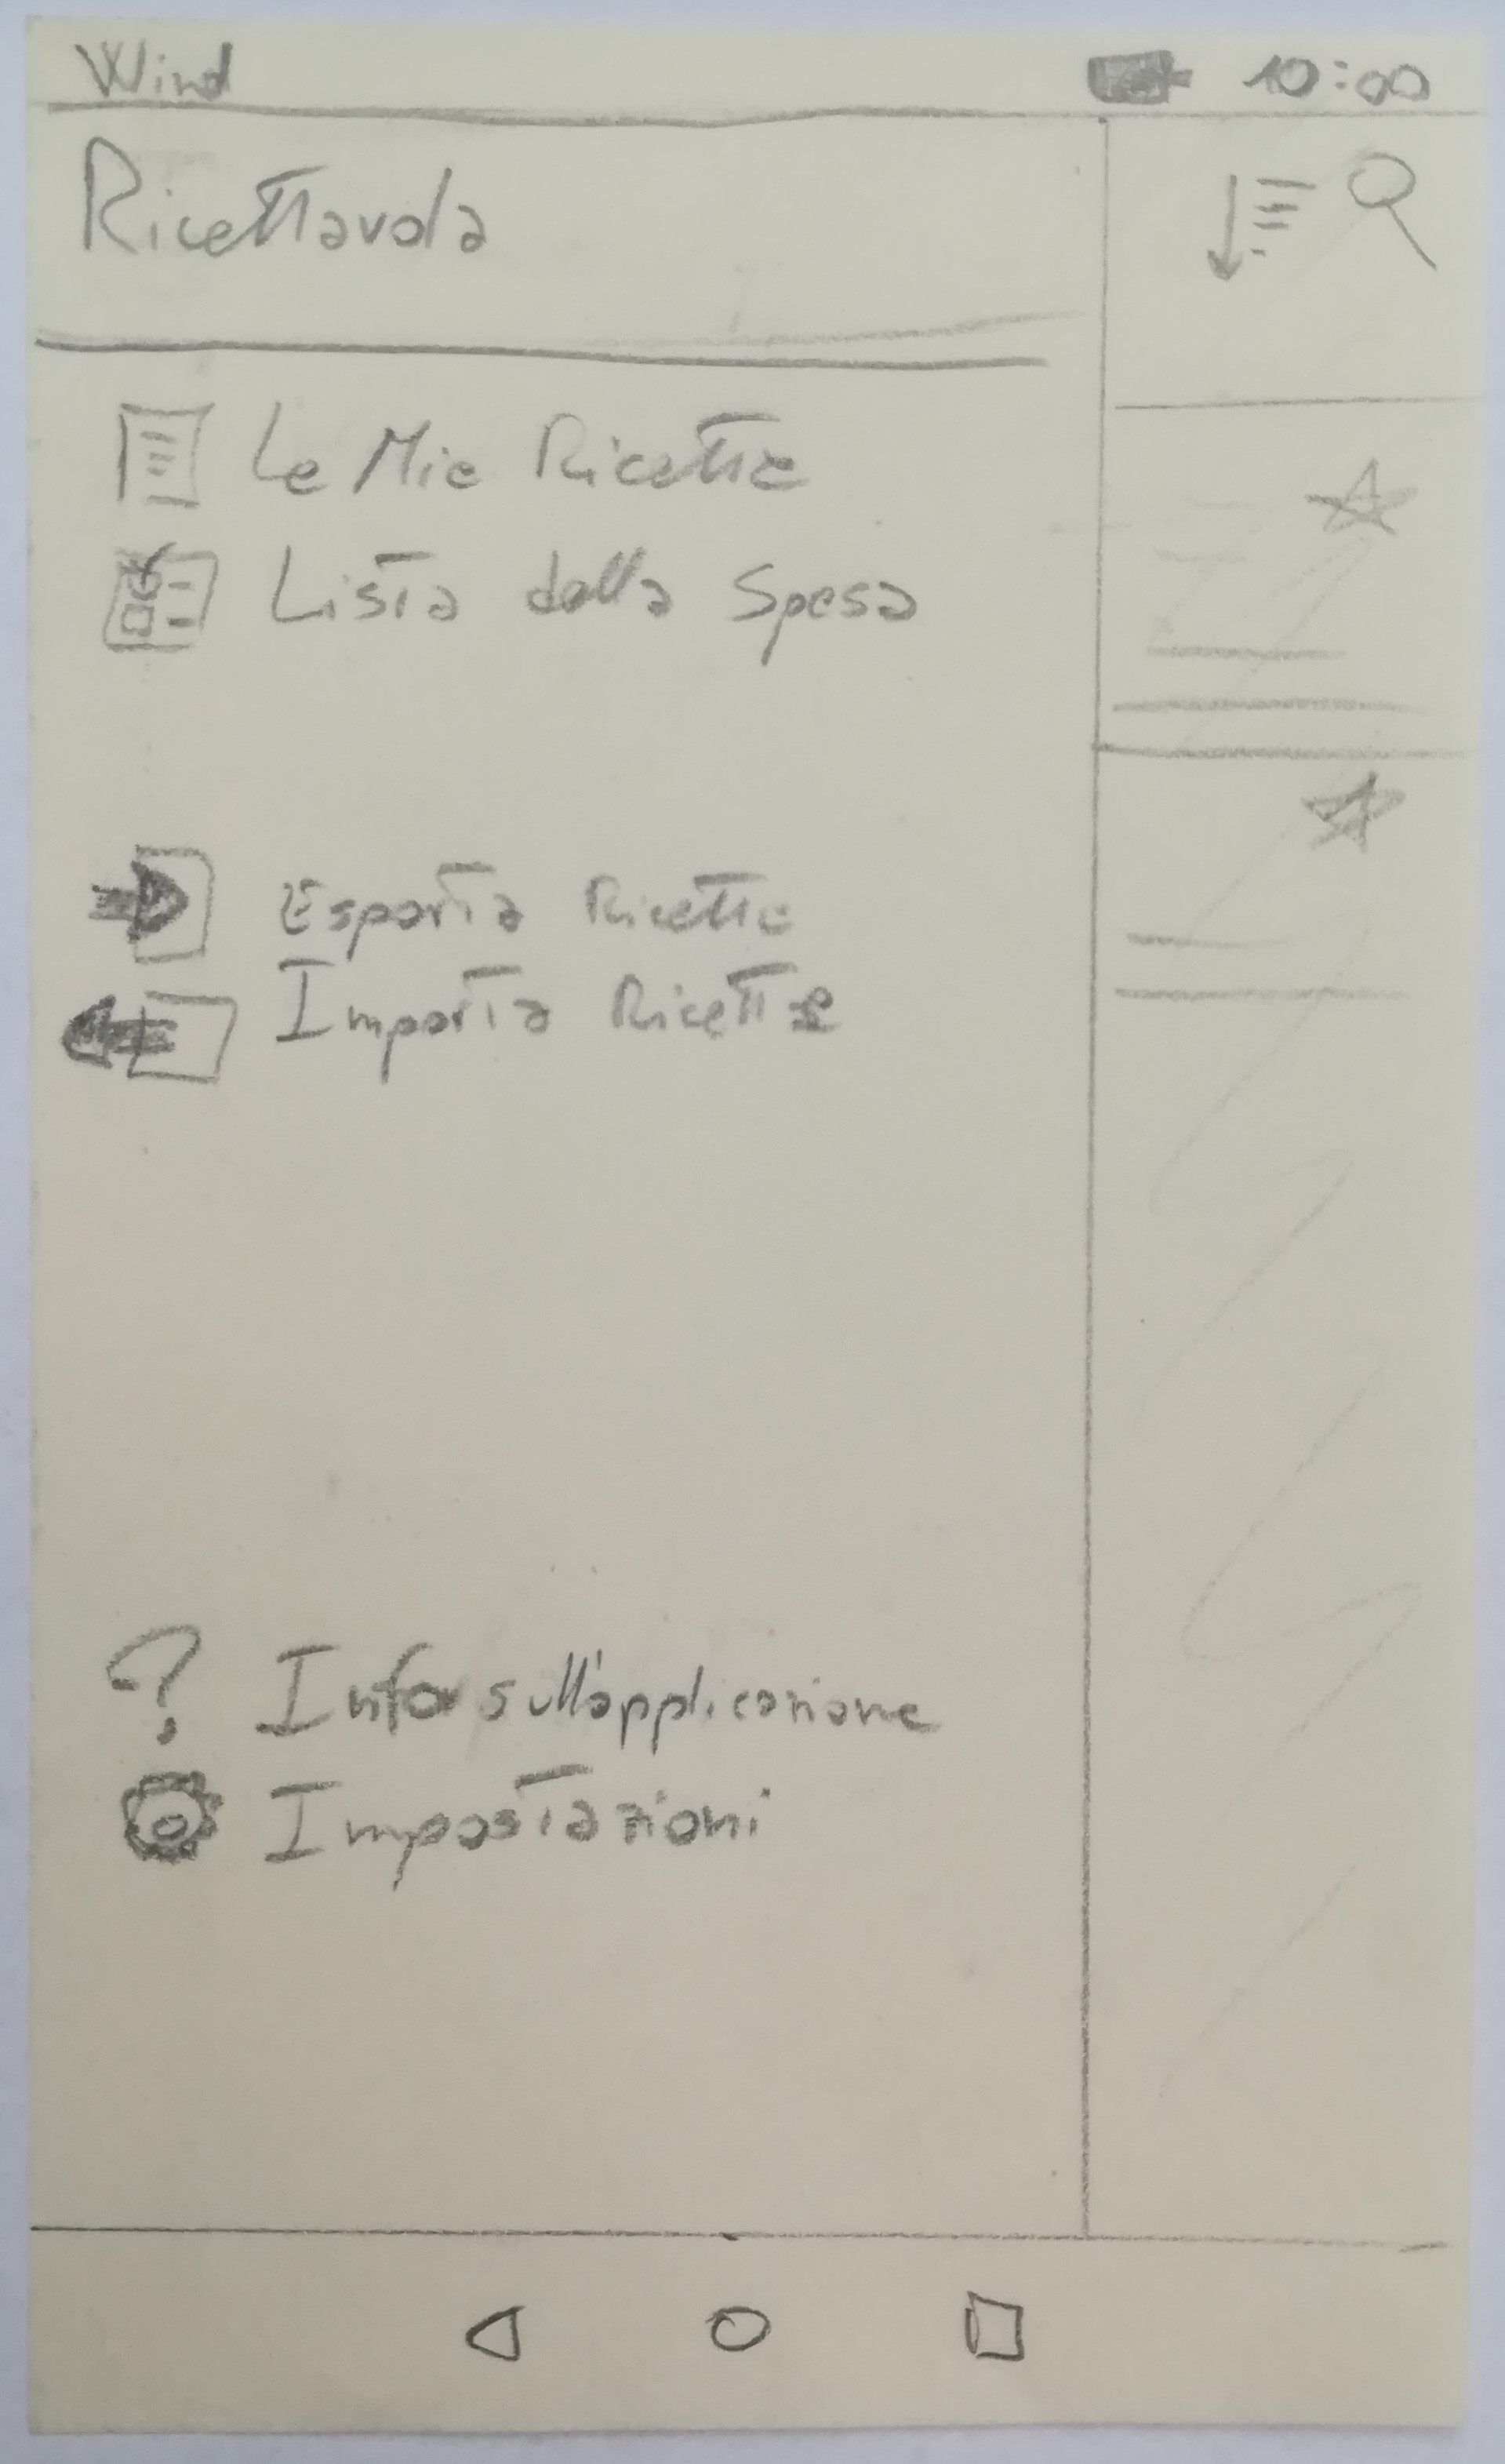
\includegraphics[width=0.47\textwidth]{prototipo1/tab_laterale}
    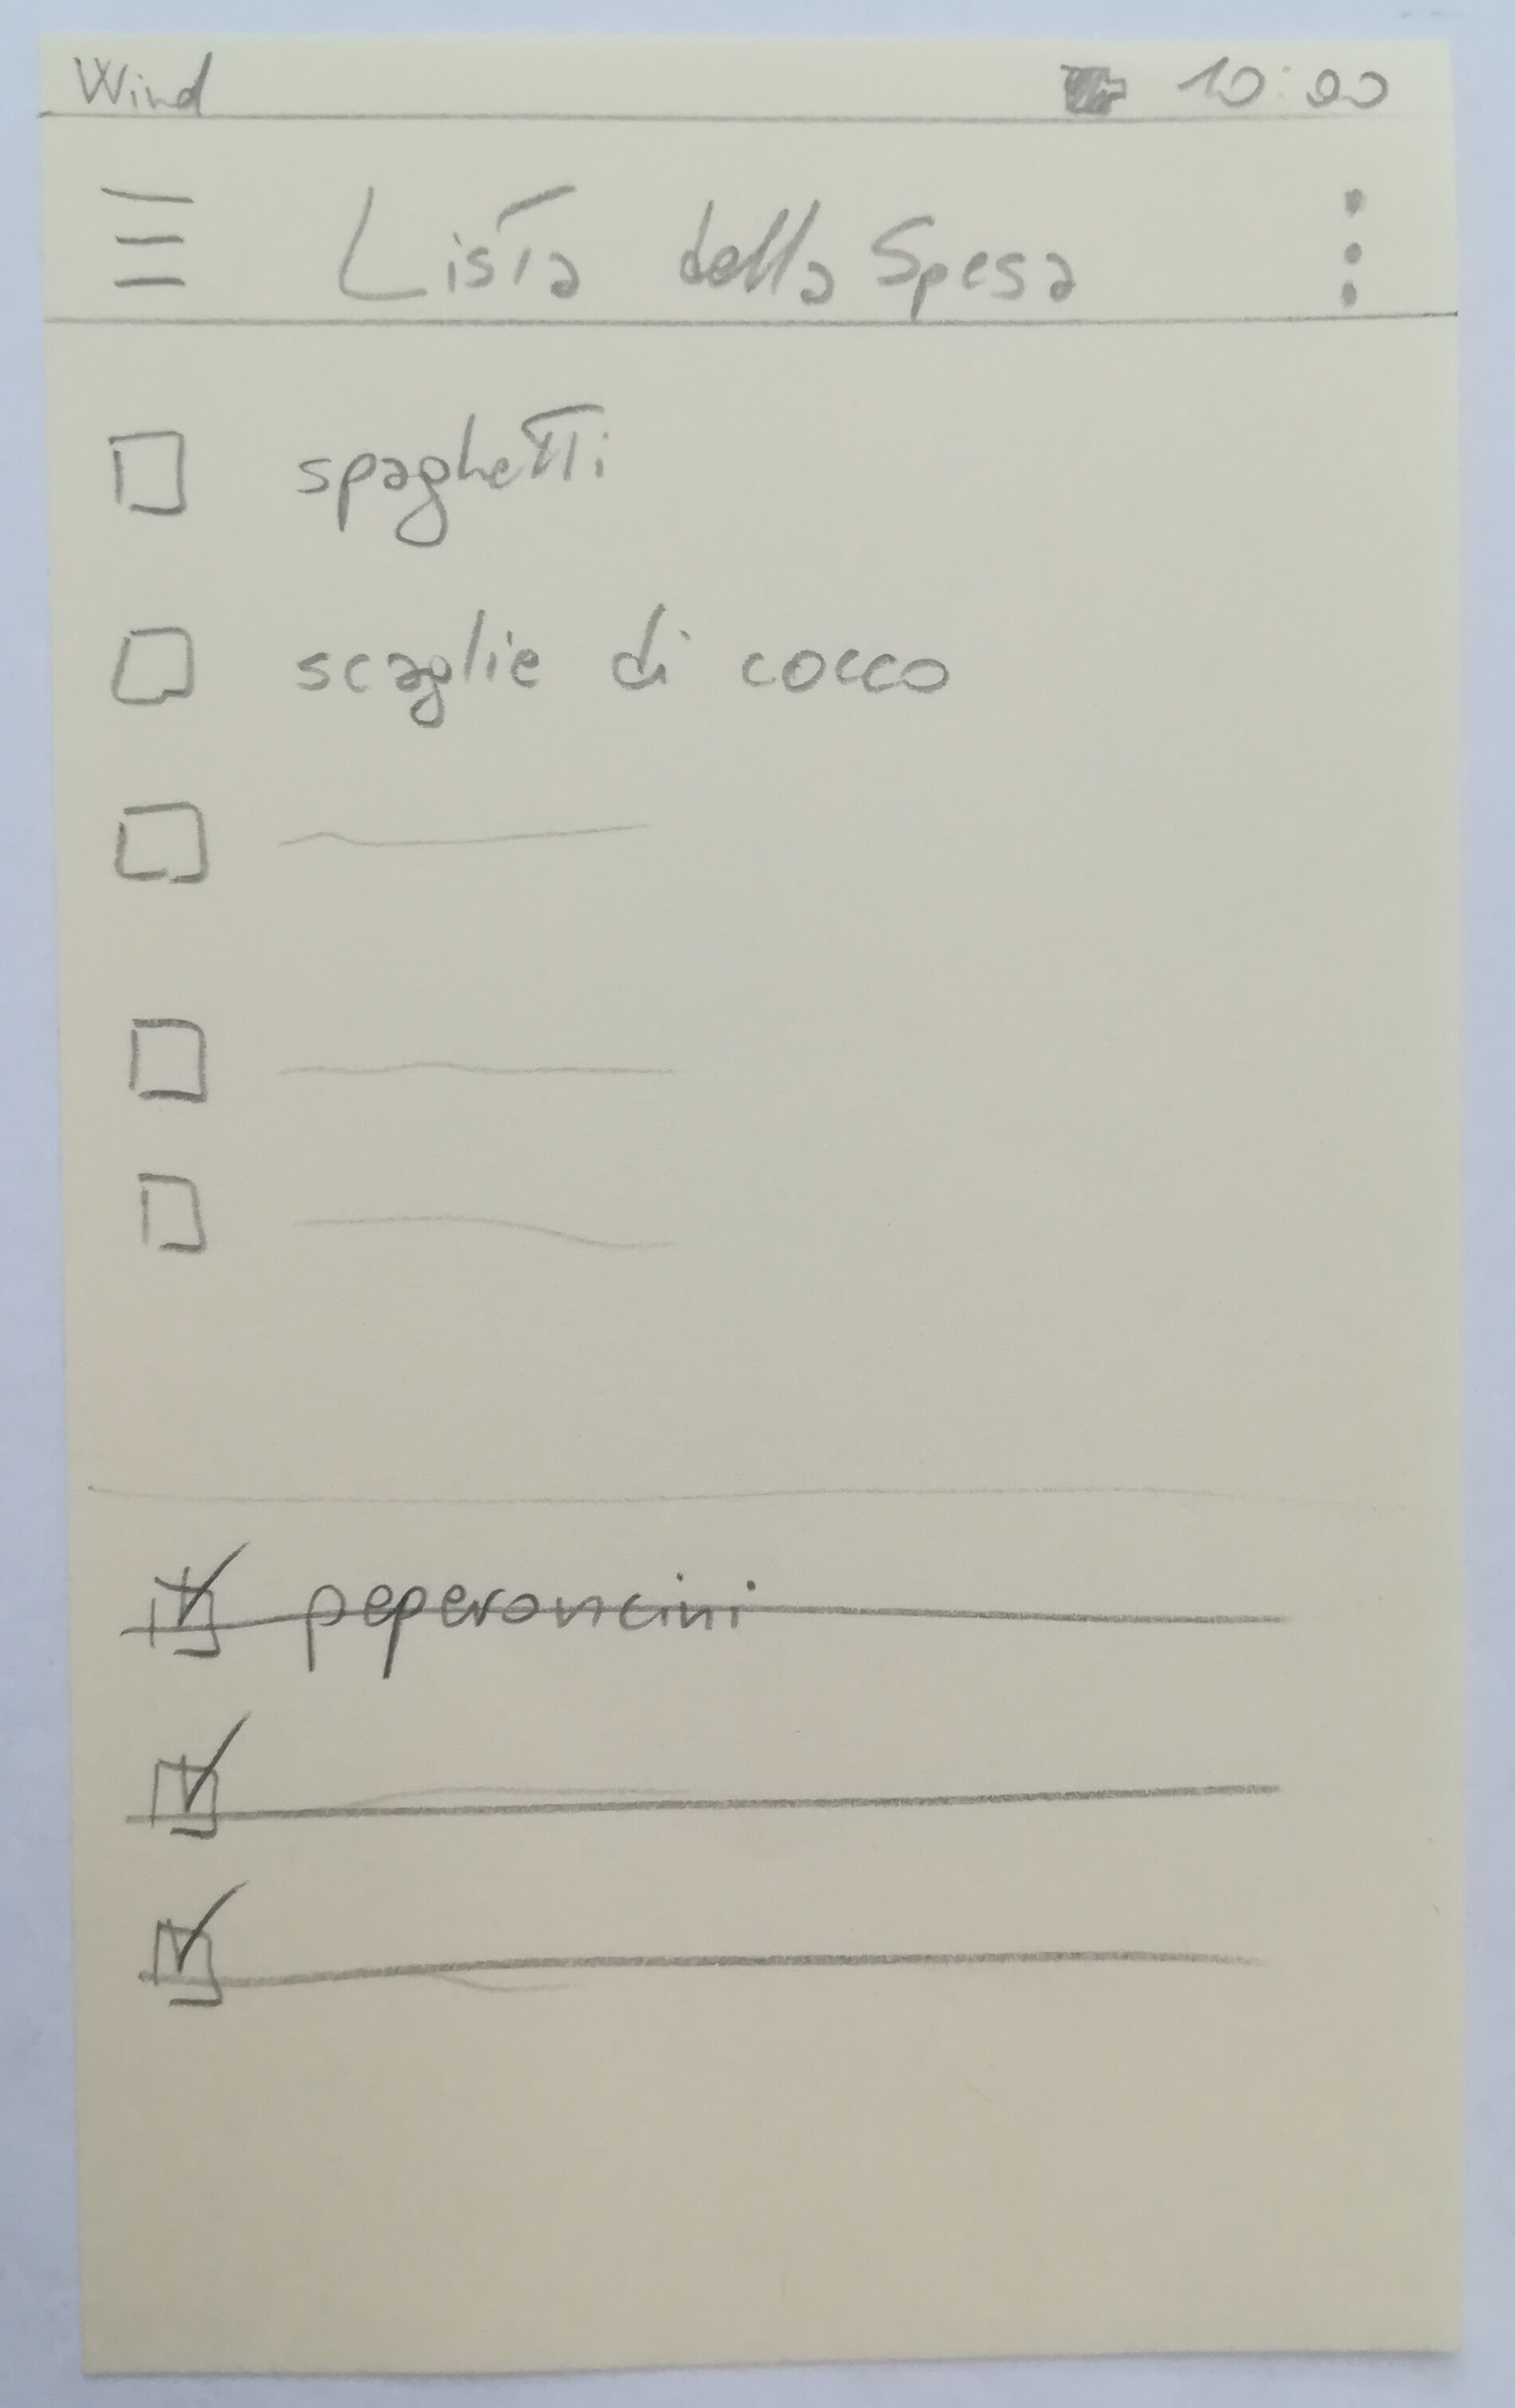
\includegraphics[width=0.49\textwidth]{prototipo1/main_lista_della_spesa}
    \caption{Da sinistra a destra: TODO laterale, la lista della spesa}
    \label{fig:p1_lista_spesa}
  \end{center}
\end{figure}


\clearpage
Dalla attività principale, premendo una ricetta, si passa alle prima schermata in figura \ref{fig:p1_ricetta}.
Nel toolbar sono presenti alcune azioni comuni, come modificare o condividere la ricetta, e ovviamente la possibilità di tornare alla schermata precedetene.
Poco sotto il toolbar sono presenti tre tab: Riepilogo, Ingredienti, Preparazione.
La prima linguetta è selezionata, infatti si possono osservare le principali informazioni della ricetta selezionata.
Premendo su una linguetta o con un'azione di \textit{swipe} si può passare alle altre schermate.
La seconda immagine mostra tutti gli ingredienti necessari, inoltre offre la possibilità di incrementare automaticamente la quantità di ingredienti in funzione del numero di persone.
L'ultima schermata illustra i passaggi numerati della ricetta.
Il tasto "Cuciamo!" in fondo allo schermo permette di avviare la modalità assistente per questa ricetta.

\begin{figure}[ht]
  \begin{center}
    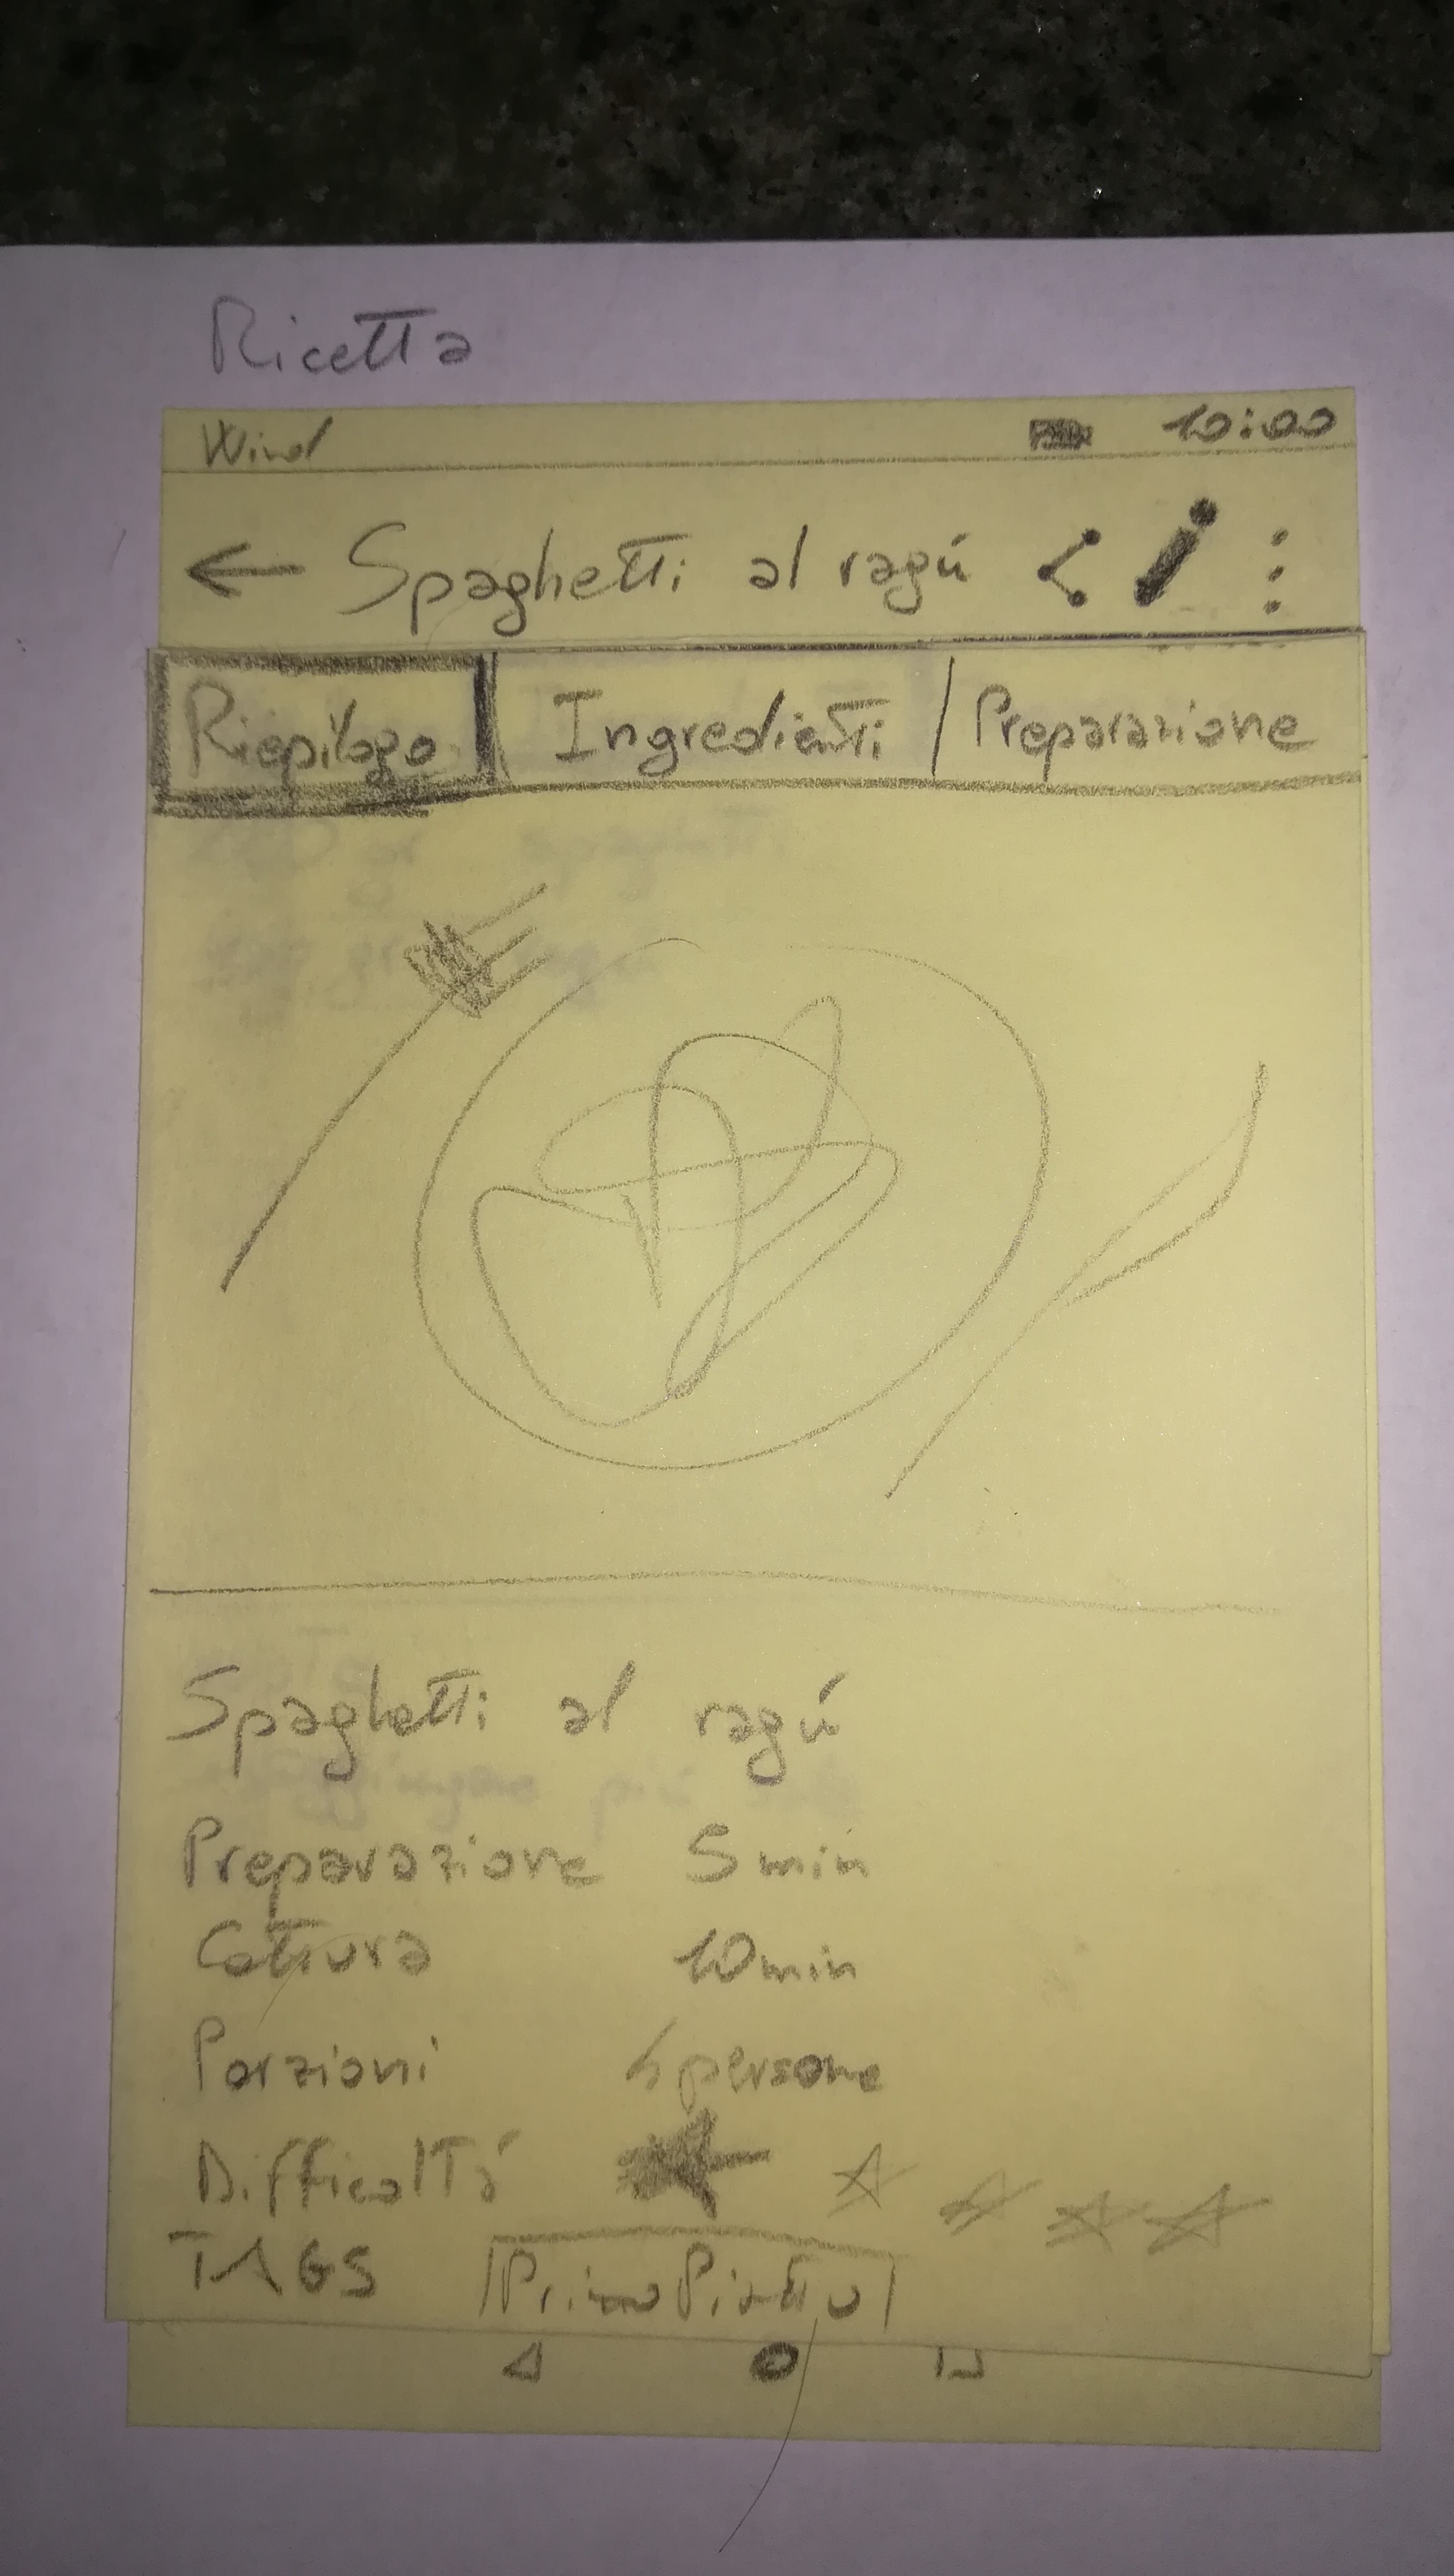
\includegraphics[width=0.325\textwidth]{prototipo1/ricetta_riepilogo}
    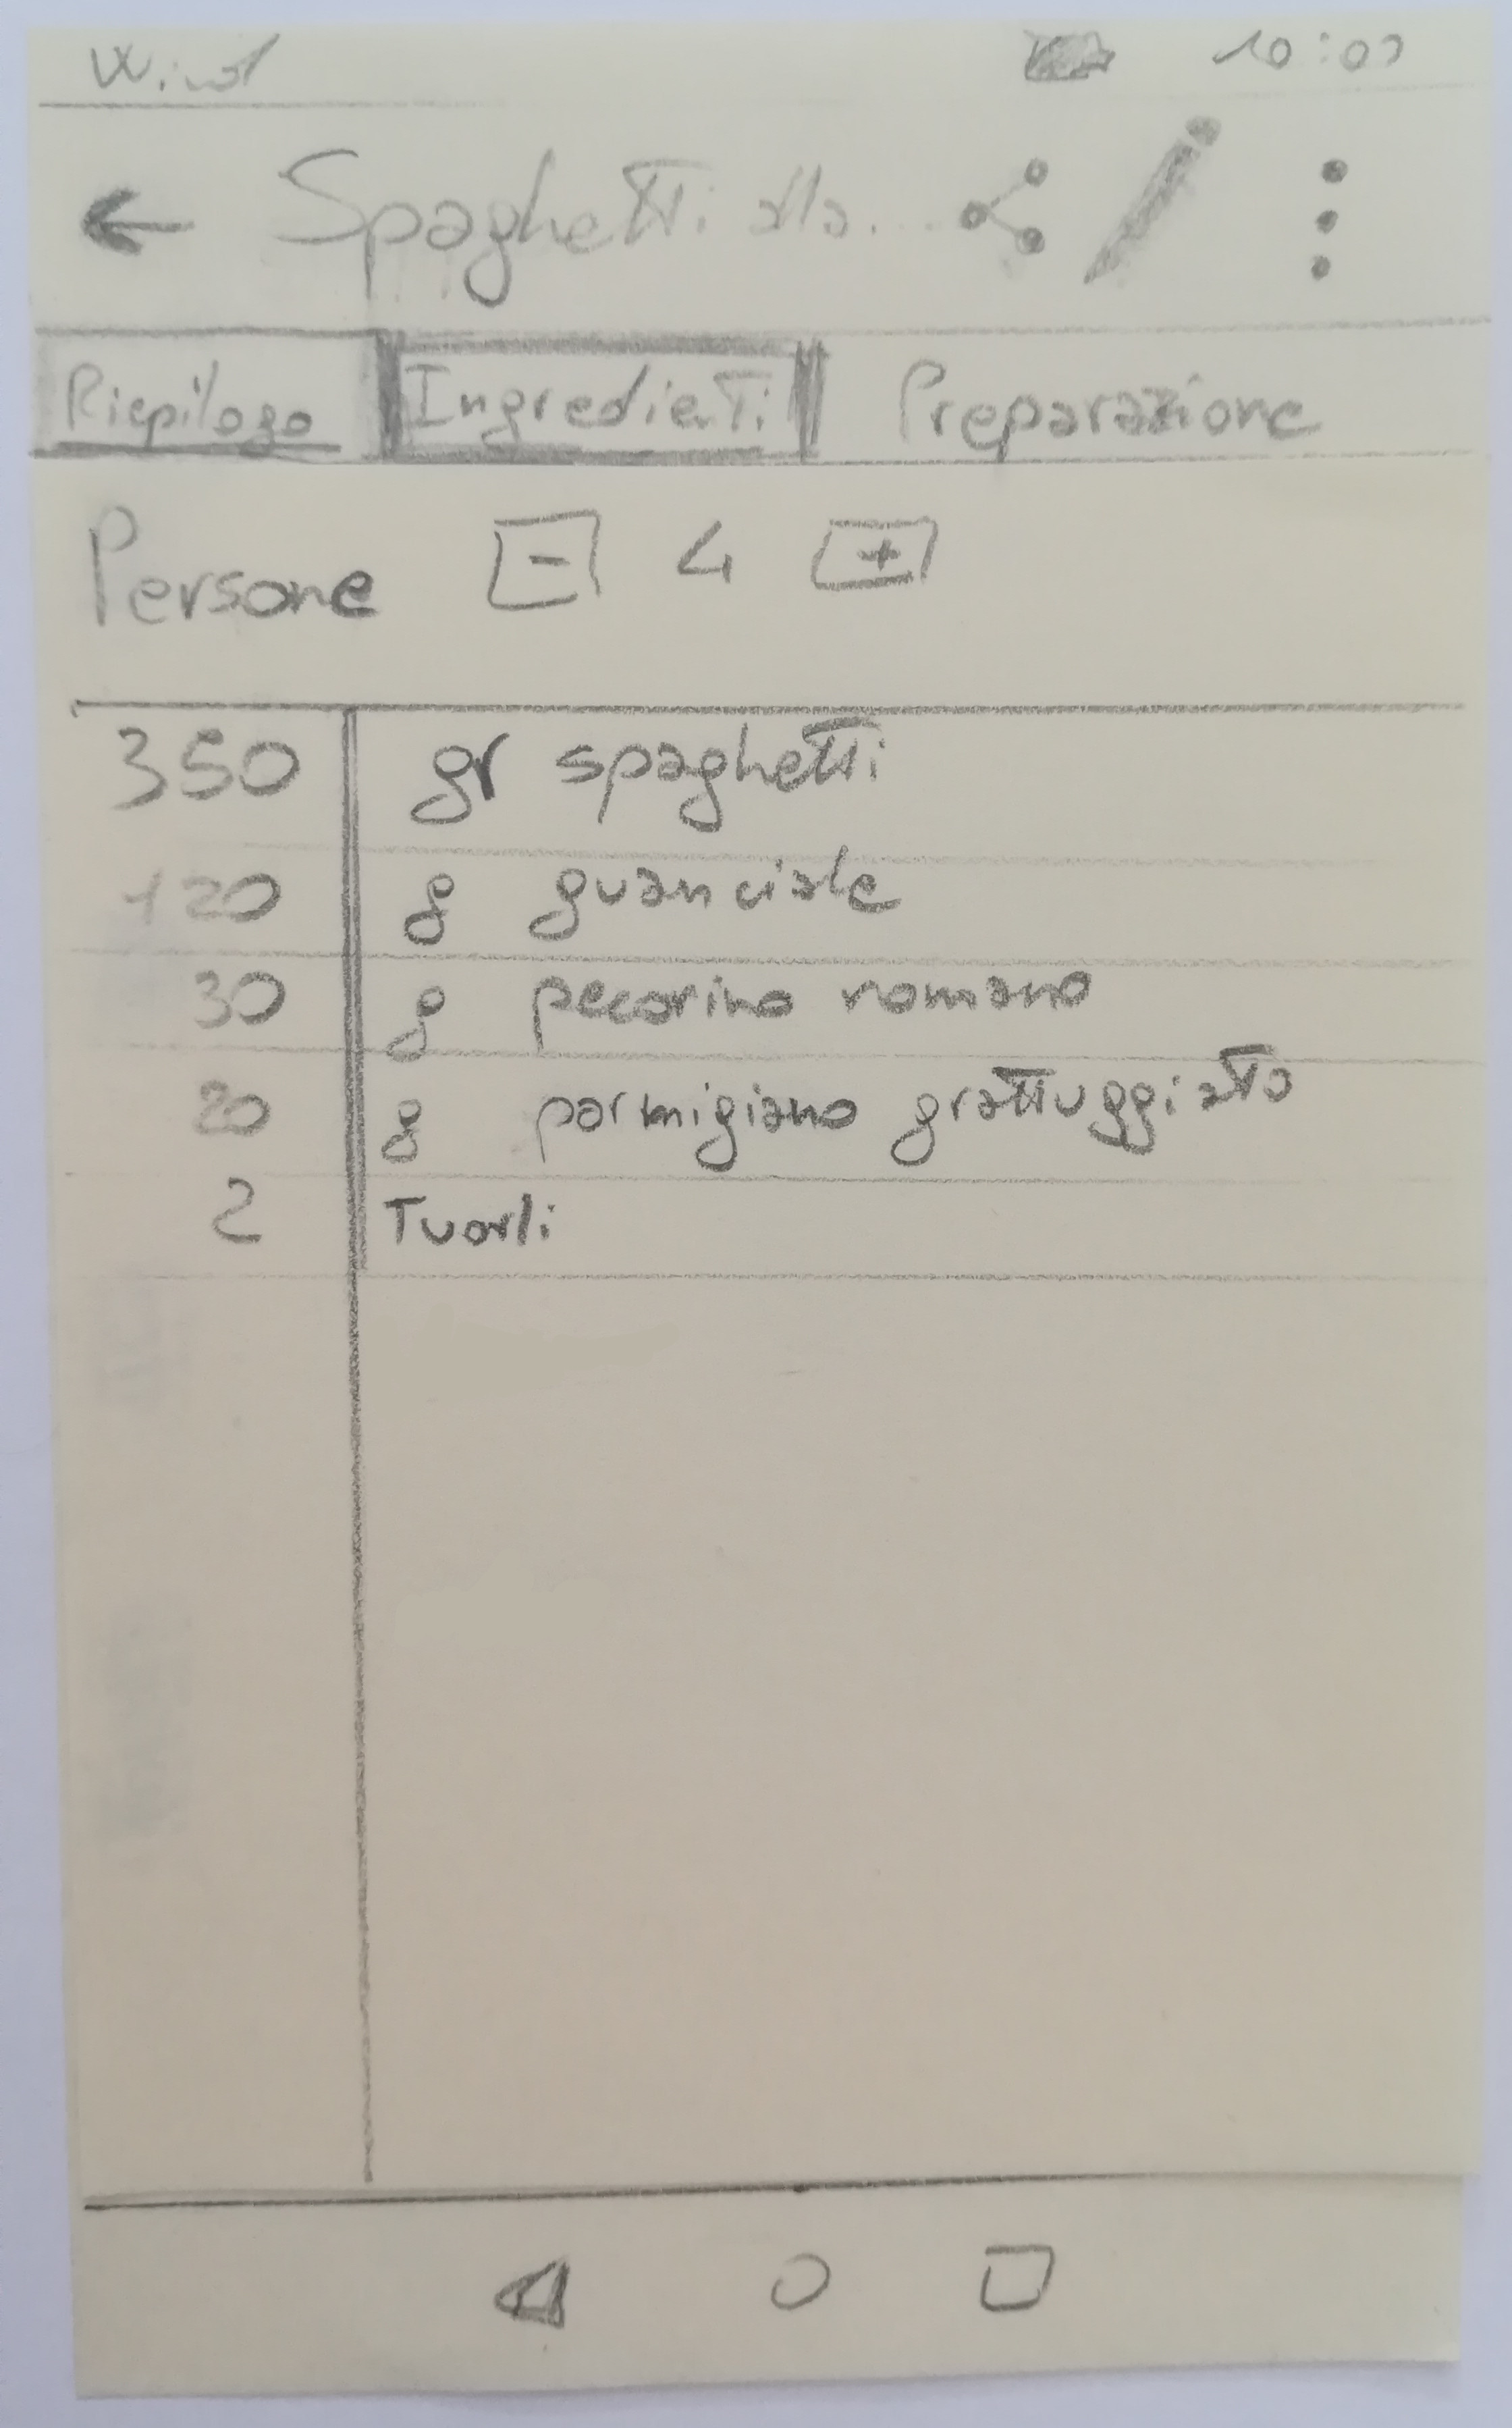
\includegraphics[width=0.325\textwidth]{prototipo1/ricetta_ingredienti}
    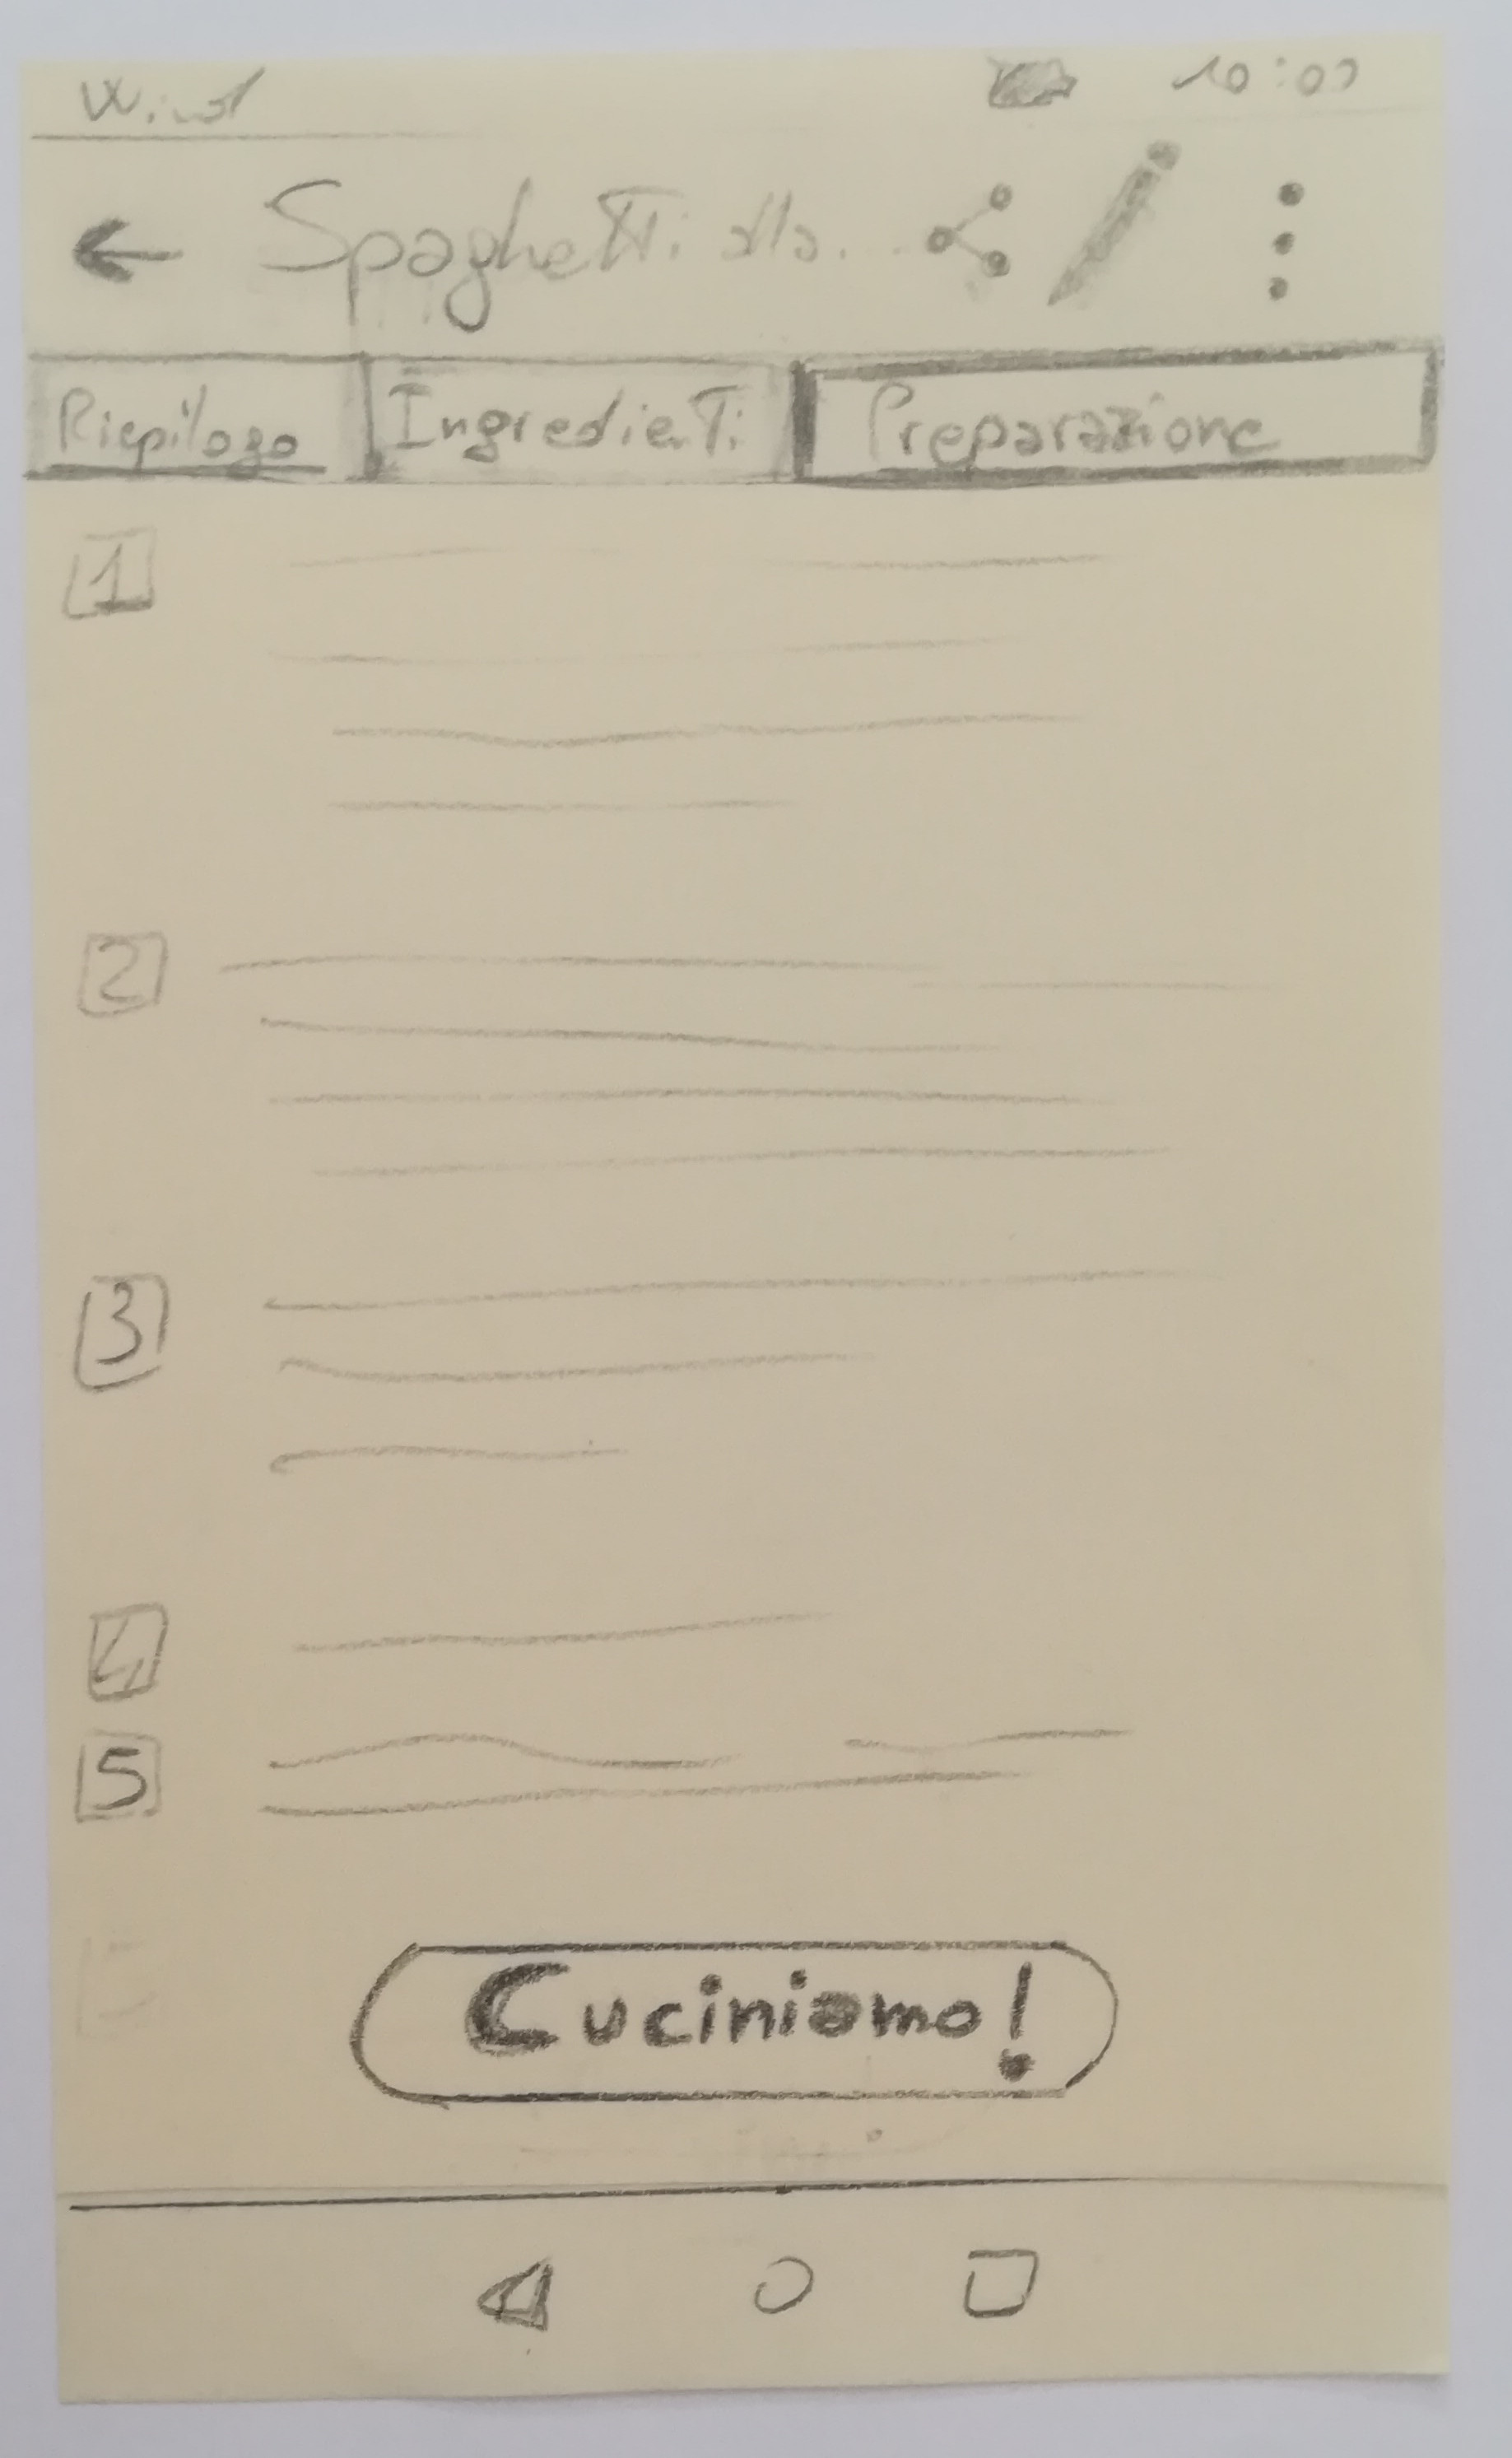
\includegraphics[width=0.325\textwidth]{prototipo1/ricetta_preparazione}
    \caption{Da sinistra a destra: riepilogo, ingredienti, preparazione}
    \label{fig:p1_ricetta}
  \end{center}
\end{figure}

\clearpage
Prima di spiegare quali sono le schermate della modalità assistente, si vuole fare una parentesi sulla modalità di modifica di una ricetta.
In figura \ref{fig:p1_edit_ricetta} si possono osservare come le schermate di figura \ref{fig:p1_ricetta} vengono modificate quando viene premuto il tasto a forma di matita.
Ovviamente anche la toolbar deve essere modificato perché essere possibile salvare la ricetta dopo averla modificata, ma non è accettabile che si voglia condividere una ricetta in fase di modifica.
La prima schermata permette di modificare il tempo di preparazione attraverso delle freccette.
Notare che ogni campo contenente testo diventa modificabile.
La possibilità di poter arrangiare l'ordine di ingredienti e passaggi della preparazione è indicato dalle tre barre orizzontali vicine ad ogni elemento delle liste.

\begin{figure}[ht]
  \begin{center}
    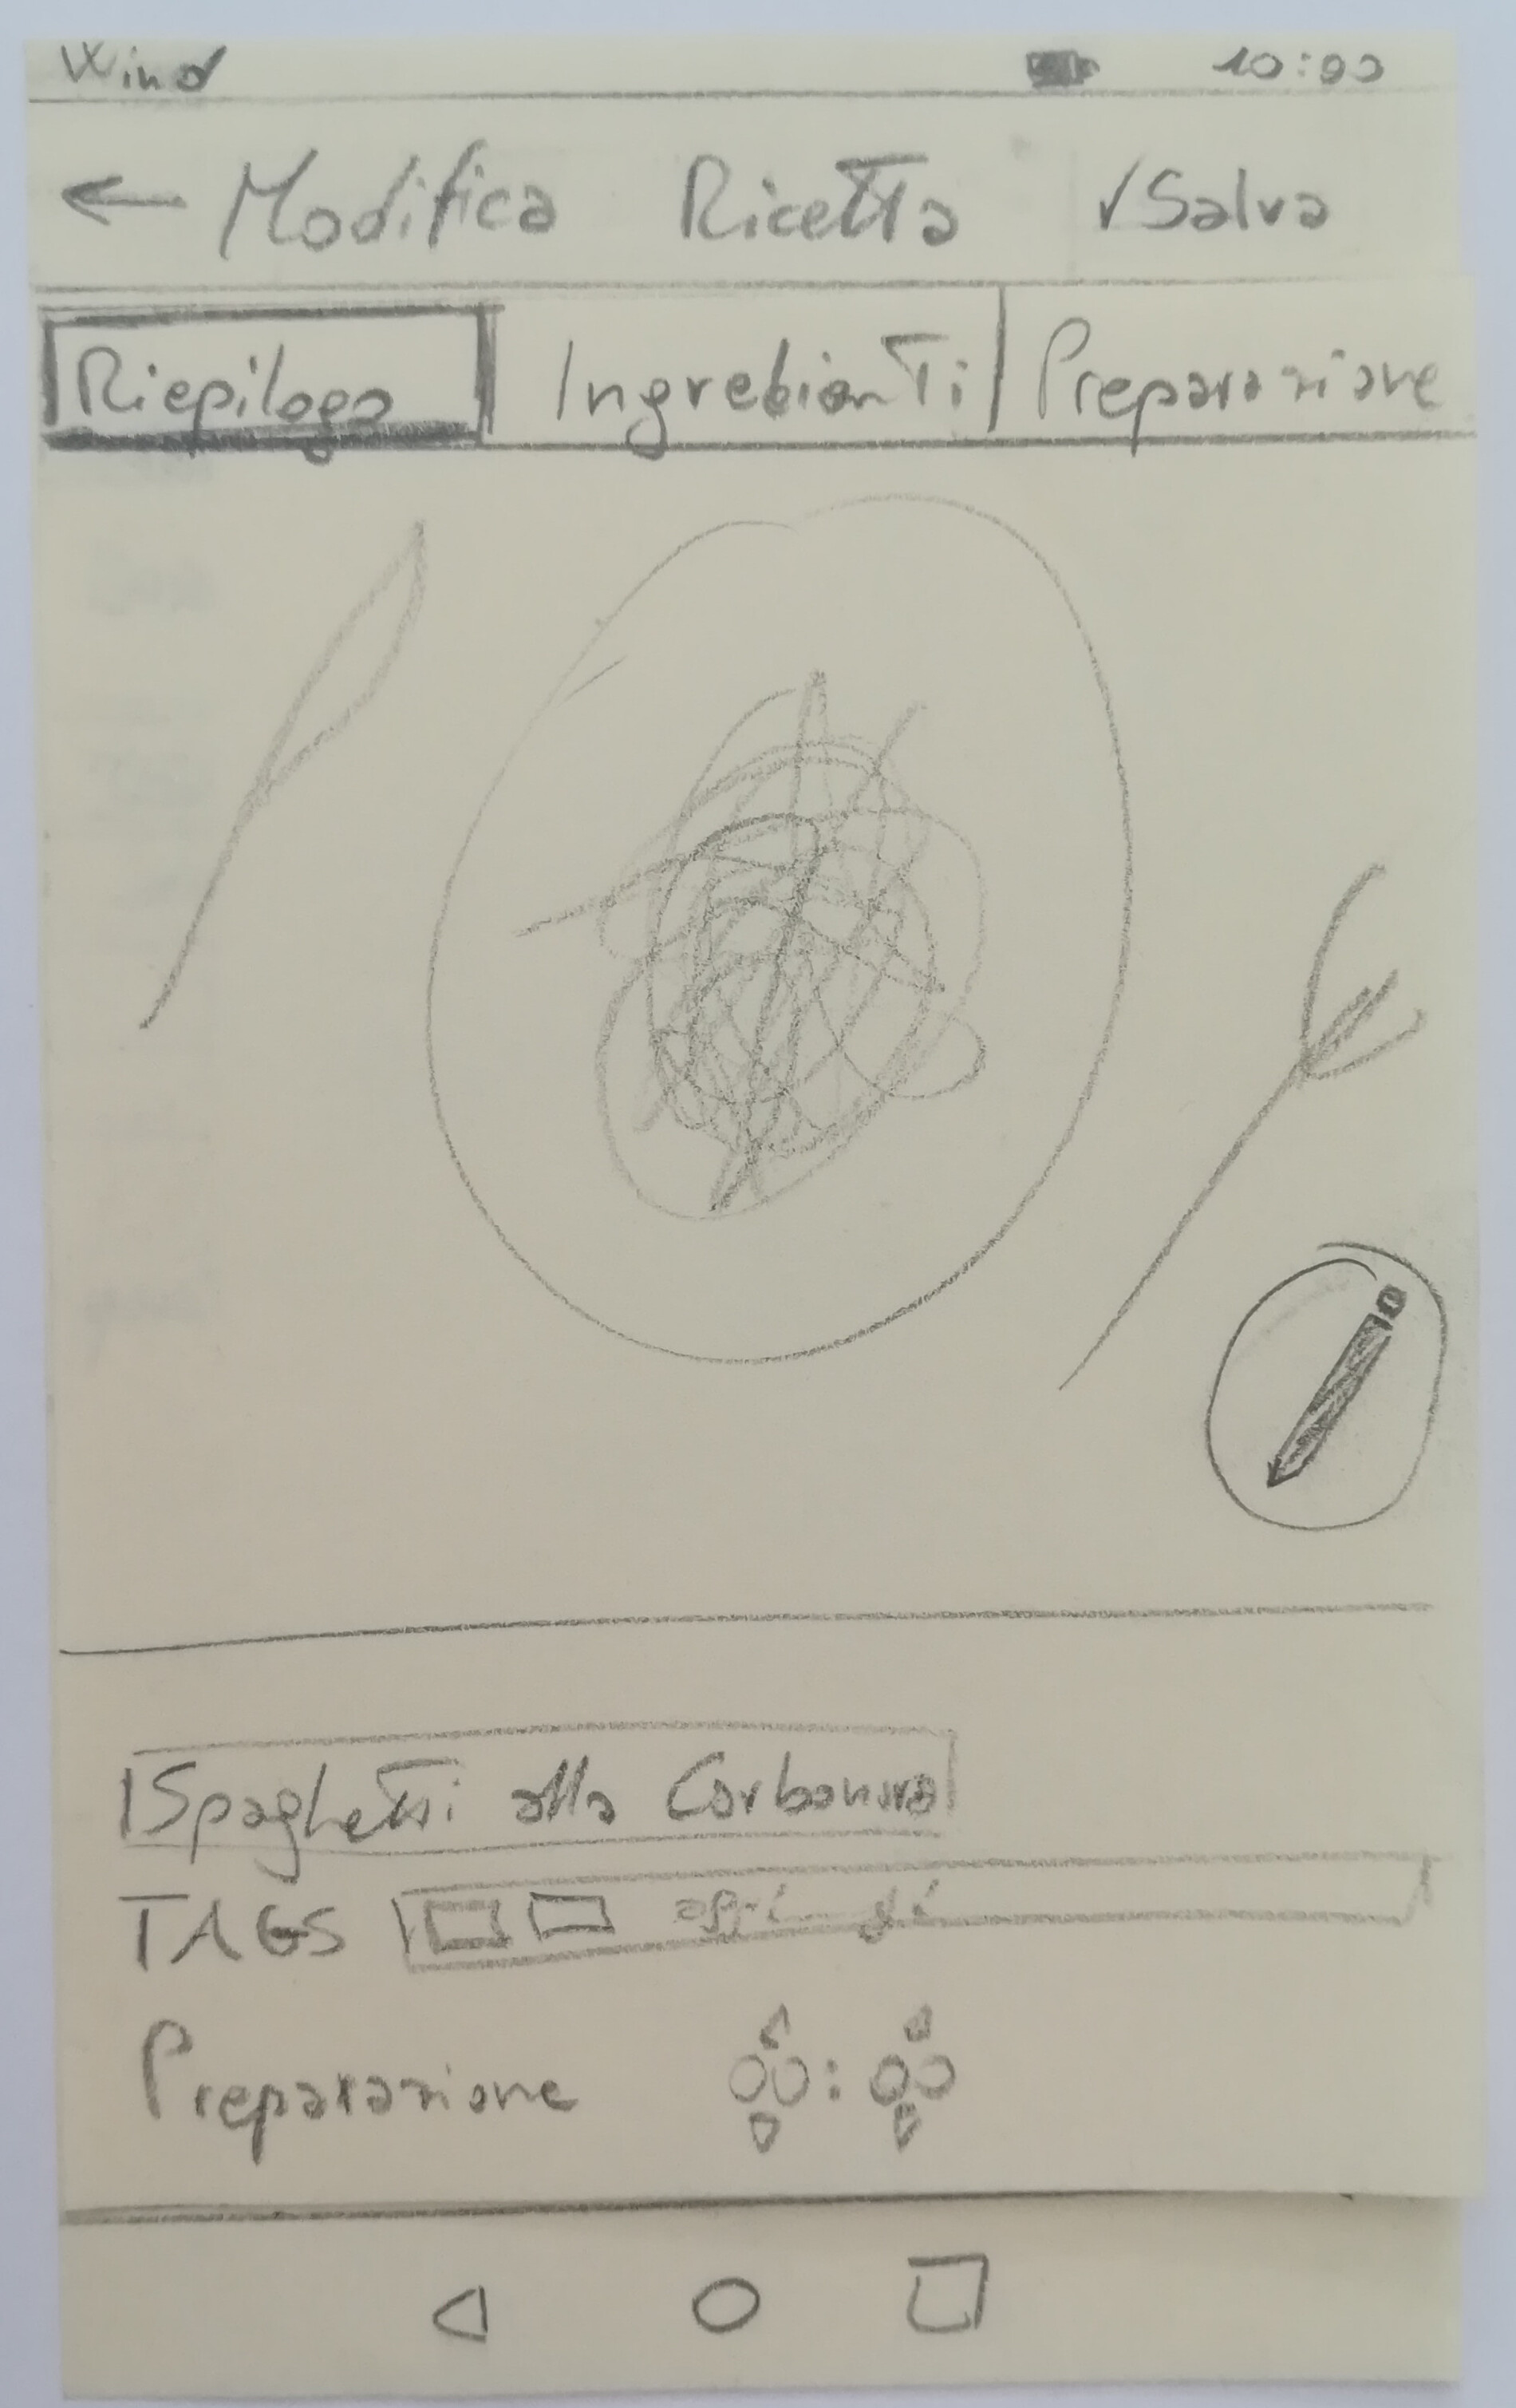
\includegraphics[width=0.325\textwidth]{prototipo1/edit_ricetta_riepilogo}
    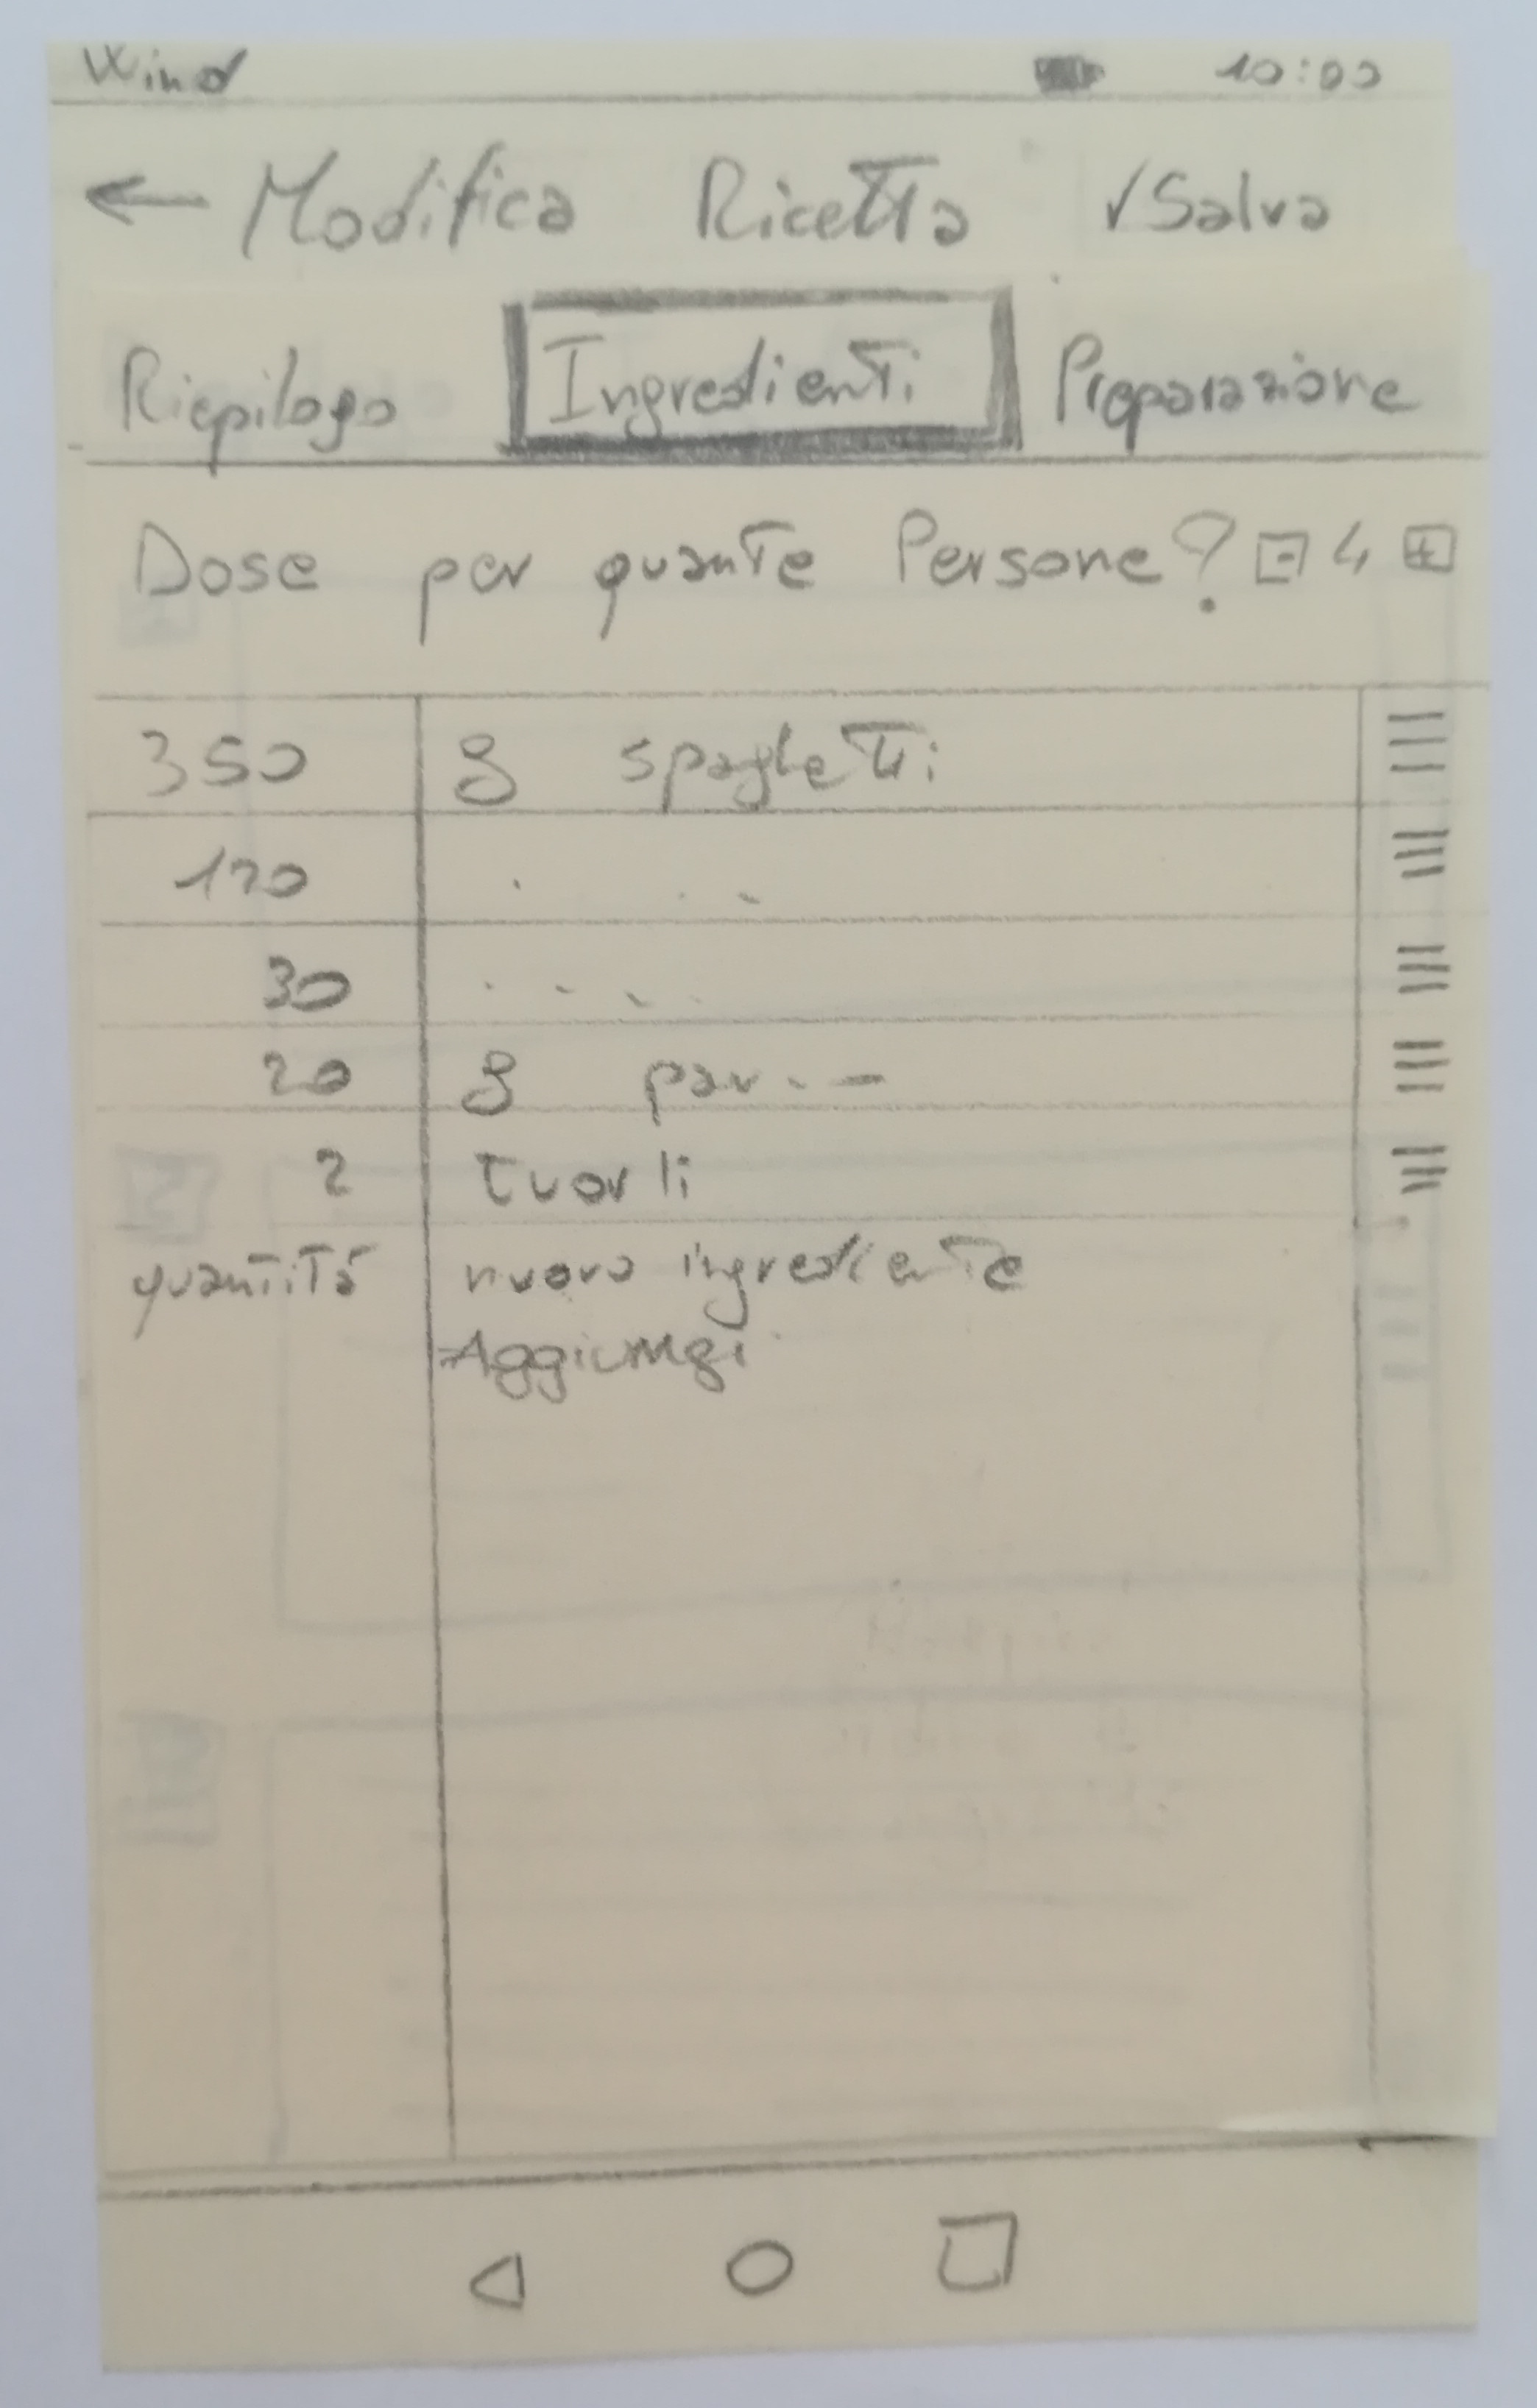
\includegraphics[width=0.325\textwidth]{prototipo1/edit_ricetta_ingredienti}
    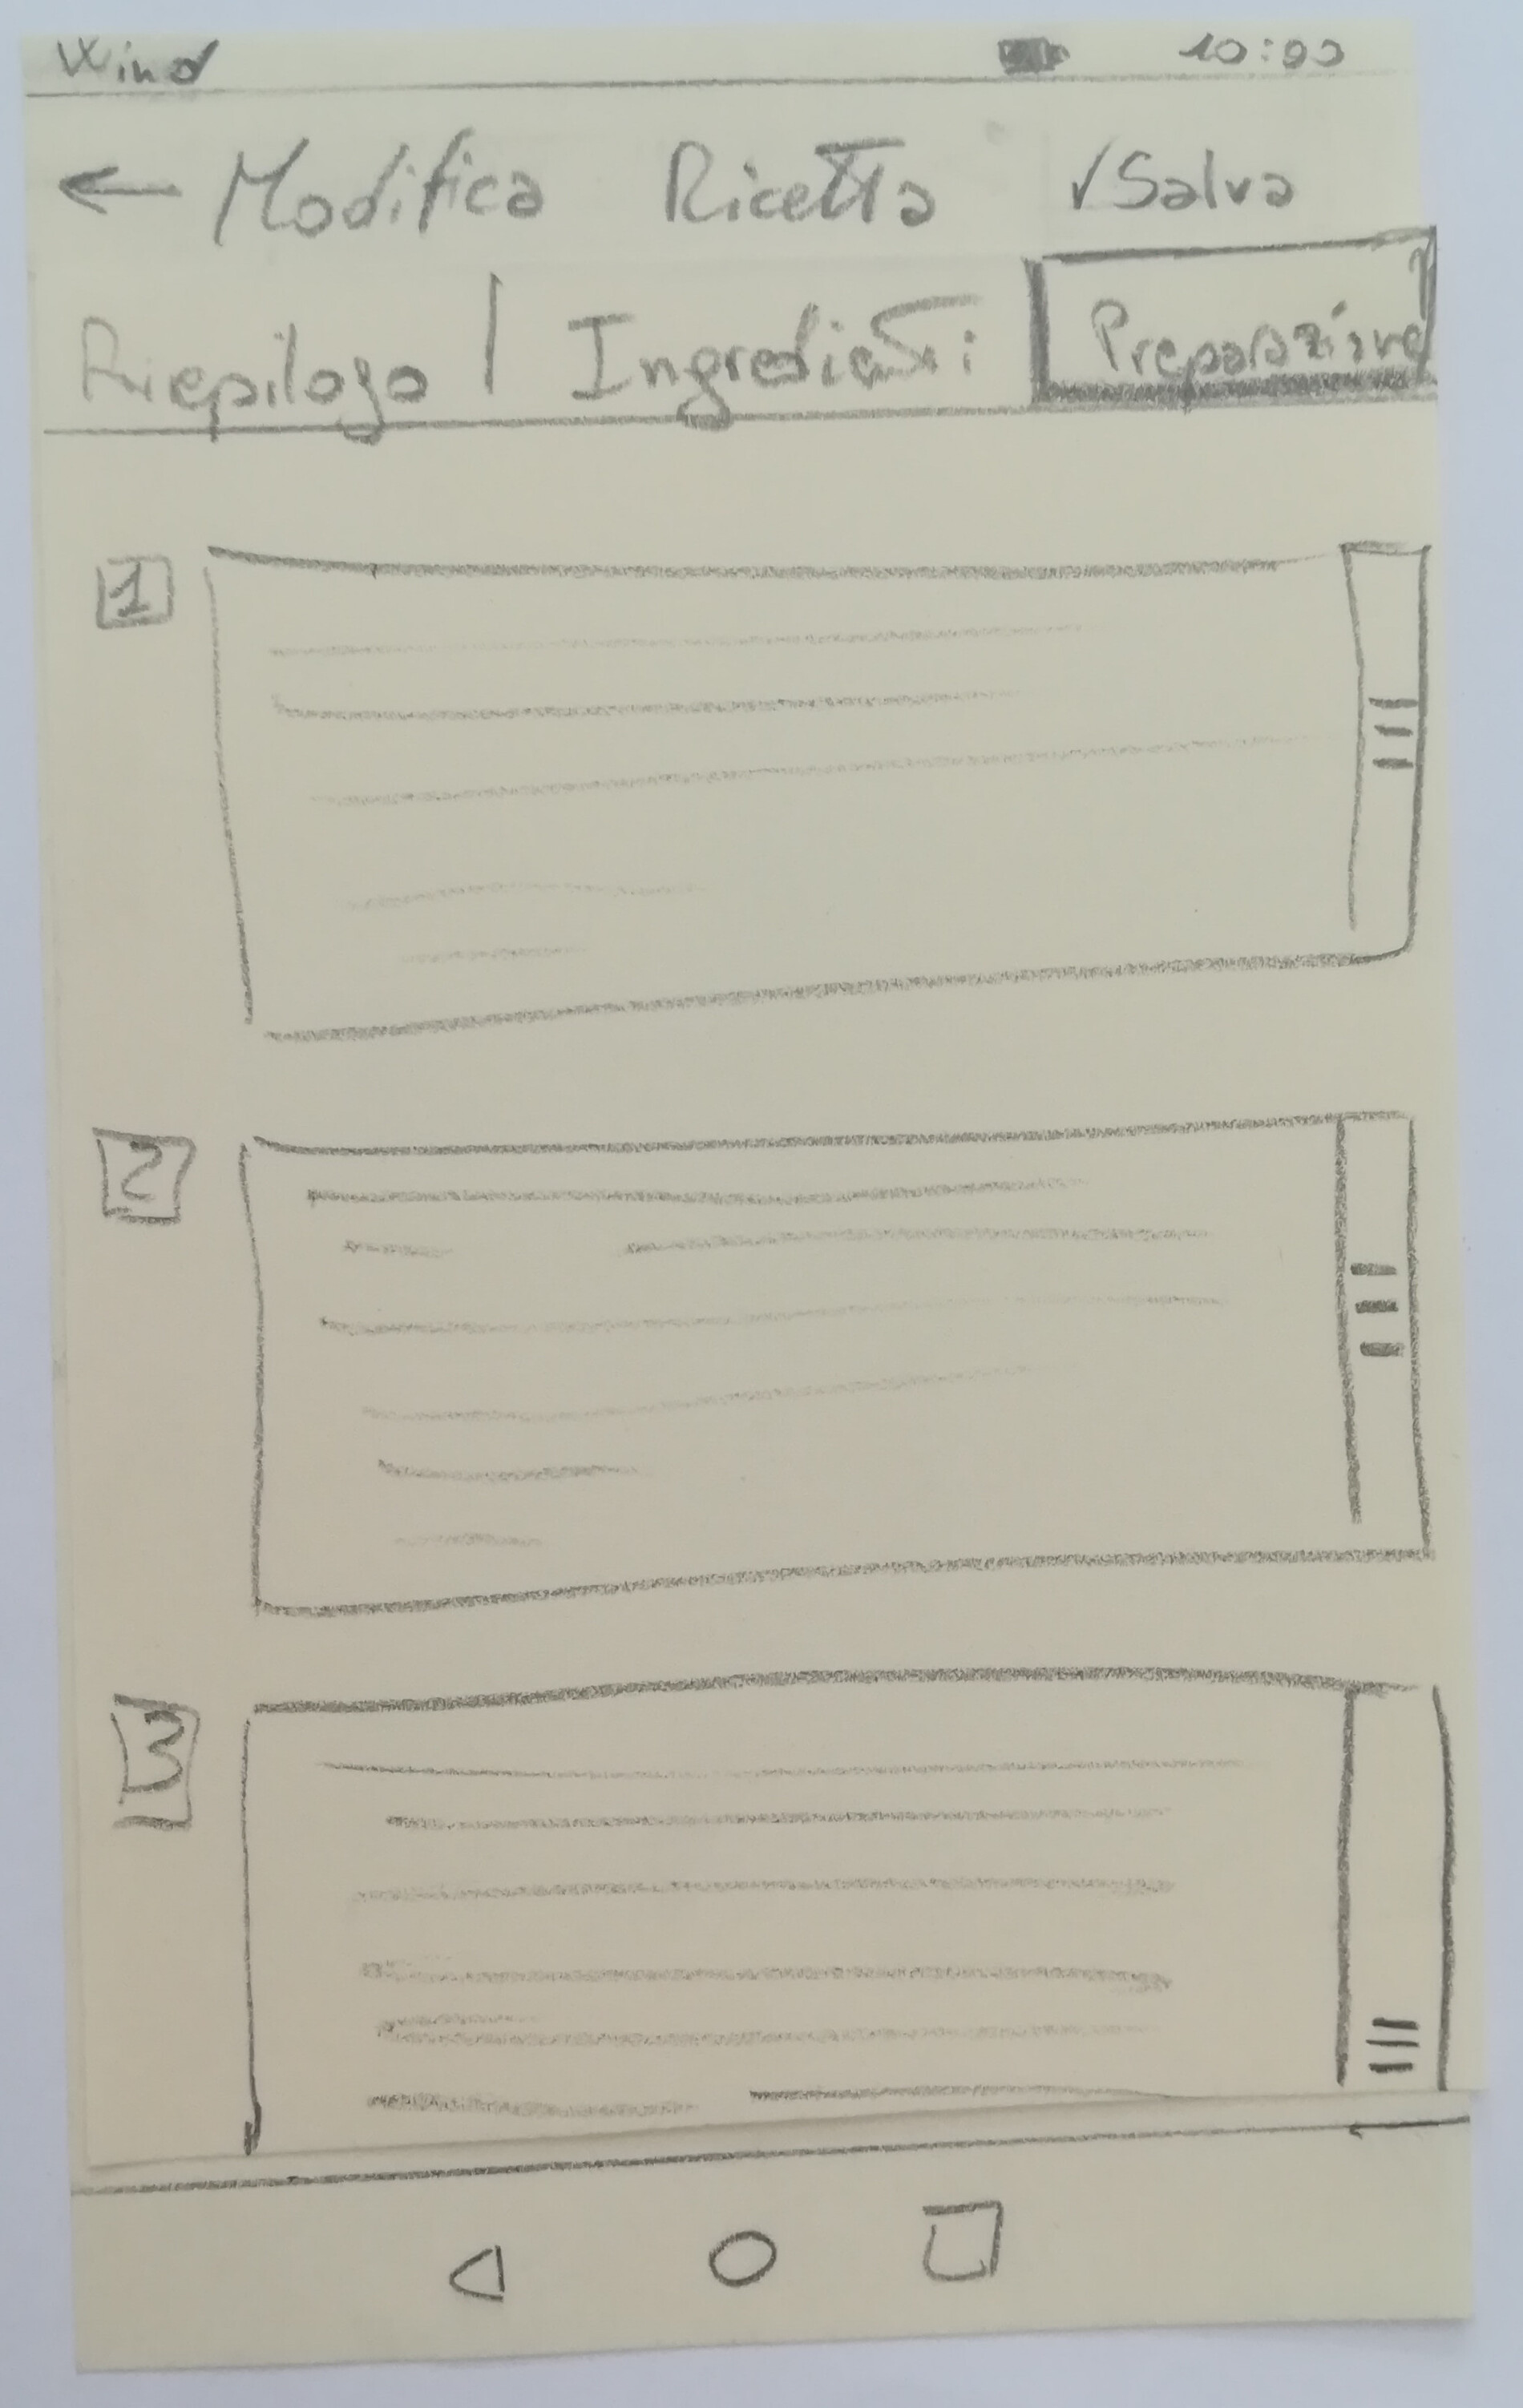
\includegraphics[width=0.325\textwidth]{prototipo1/edit_ricetta_preparazione}
    \caption{Da sinistra a destra: riepilogo, ingredienti, preparazione}
    \label{fig:p1_edit_ricetta}
  \end{center}
\end{figure}


In figura \ref{fig:p1_cuciniamo} sono mostrate tre versioni differenti della schermata assistente.
Innanzitutto si fa notare che le queste schermate sono pensate per essere usate esclusivamente in modalità \textit{landscape}.
Questa scelta è stata fatta per tentare di massimizzare la dimensione del testo nella schermata, così che fosse facilmente leggibile anche da una certa distanza.
Un altro punto in comune fra le schermate è quello di presentare due tasti ben visibili per procedere al prossimo passo oppure per rileggere quelli già effettuati.
Il criterio con cui questi tasti sono stati creati è quello di permettere all'utente di spostarsi tra i passaggi della ricetta sporcando soltanto due zone dello schermo.
Si può ipotizzare infatti che chi cucina abbia le mani bagnate o sporche di pasta, con i due tasti appena descritti si vuole minimizzare l'area toccata con le dita.
Ogni schermata presenta in alto il numero dello step corrente.
È sembrato utile integrare questa schermata con un timer, così da averlo sempre a portata di mano.

La seconda schermata ha una funzione in più rispetto alle altre perché permette di osservare, nel riquadro sotto a quello dell'orologio, gli ingredienti della ricetta.

\clearpage
\begin{figure}[ht]
  \begin{center}
    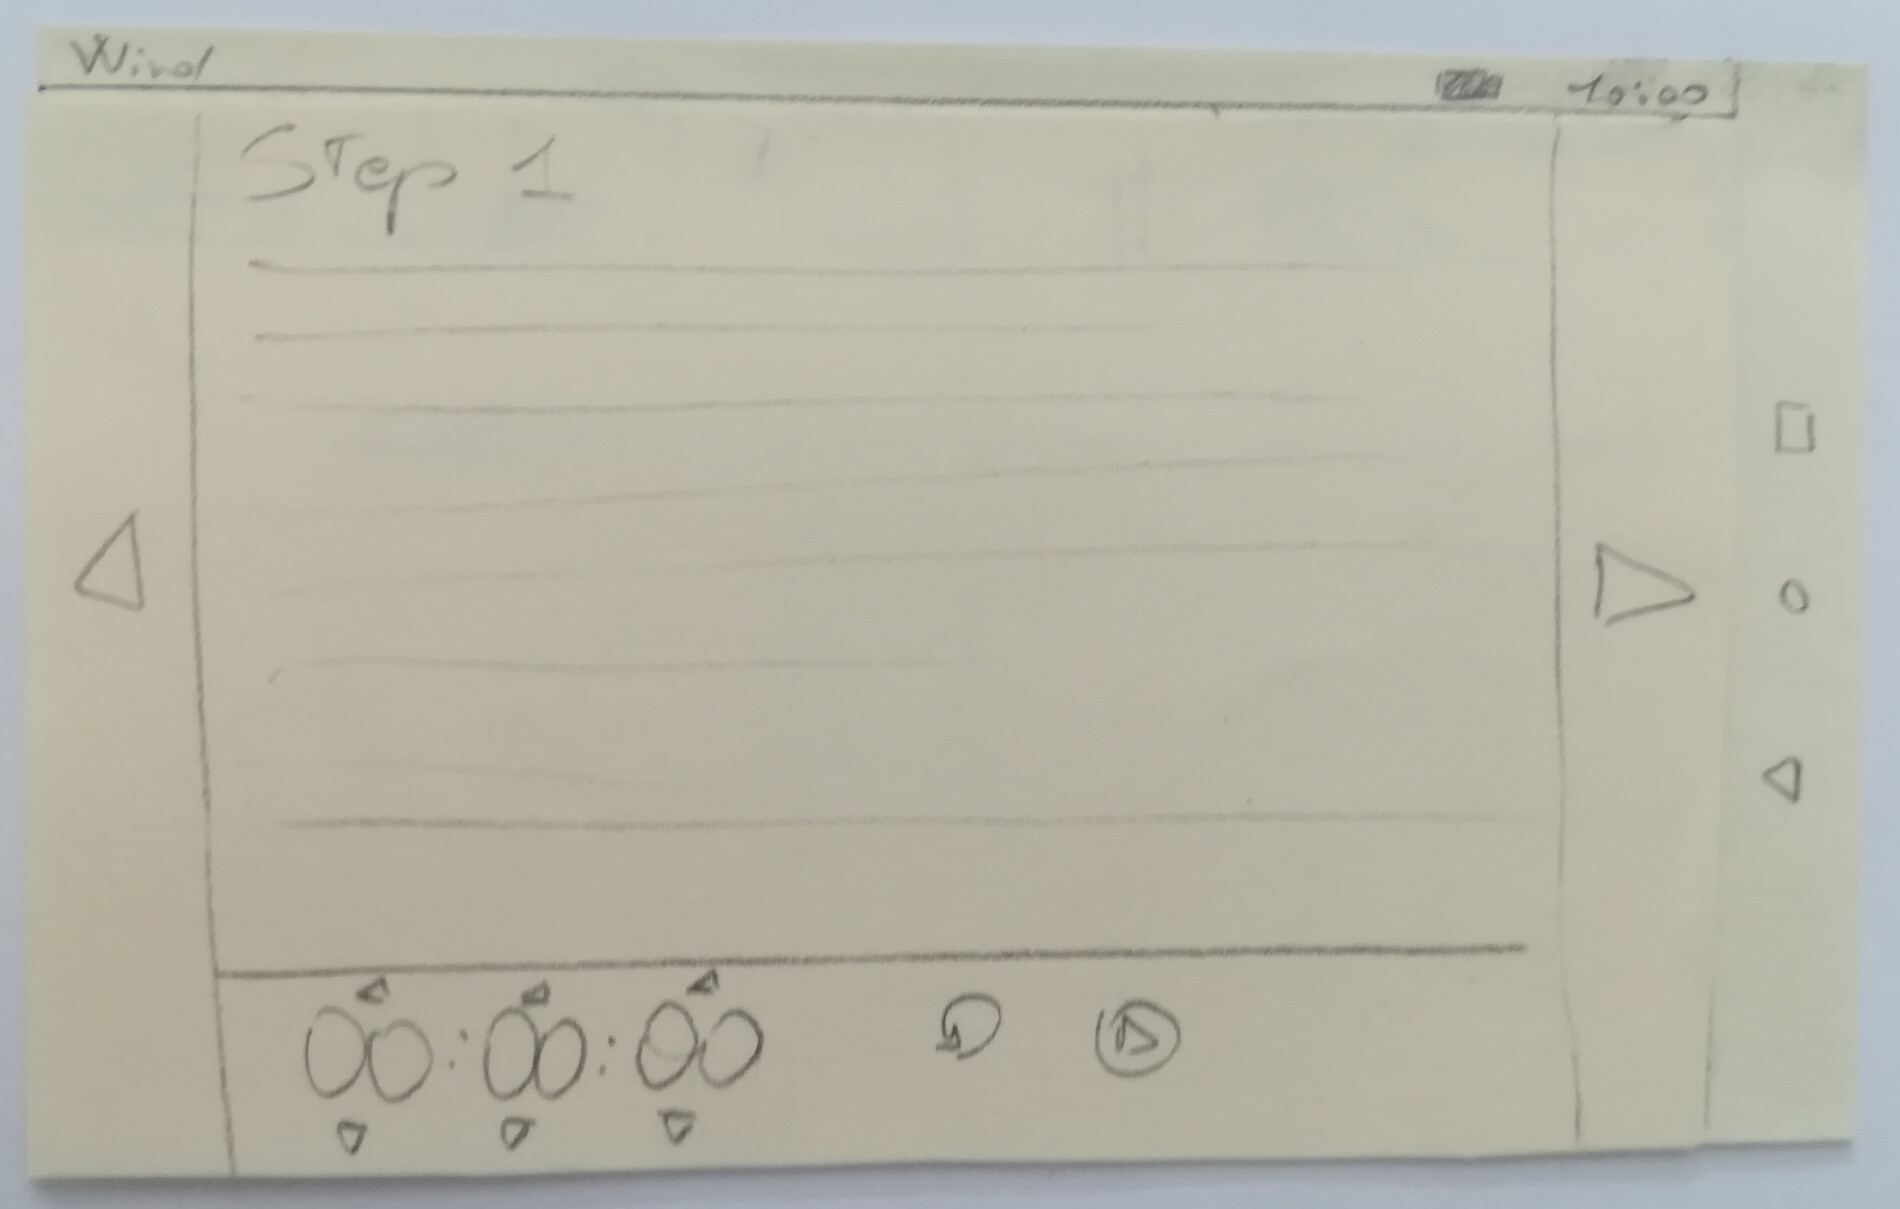
\includegraphics[width=0.78\textwidth]{prototipo1/cuciamo_a}
    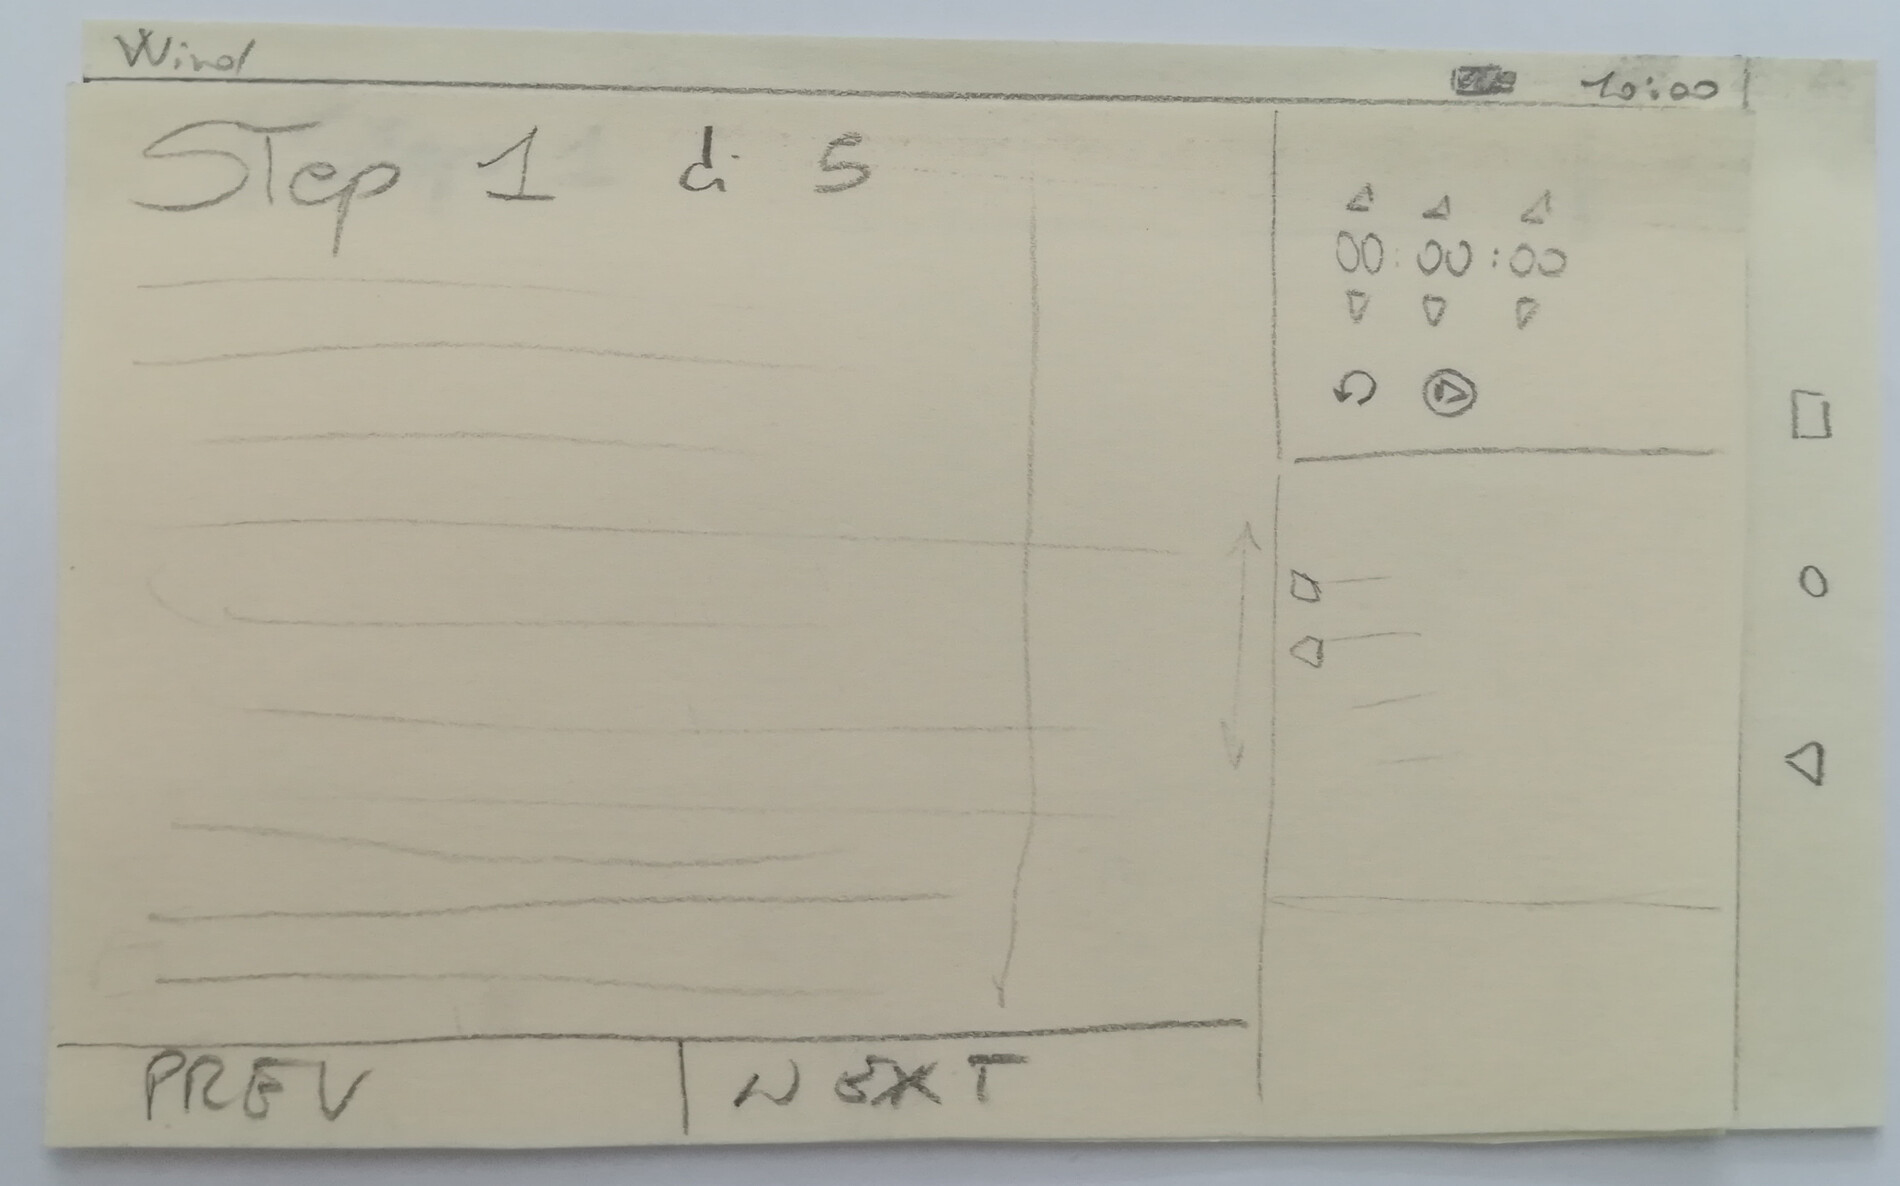
\includegraphics[width=0.78\textwidth]{prototipo1/cuciamo_b}
    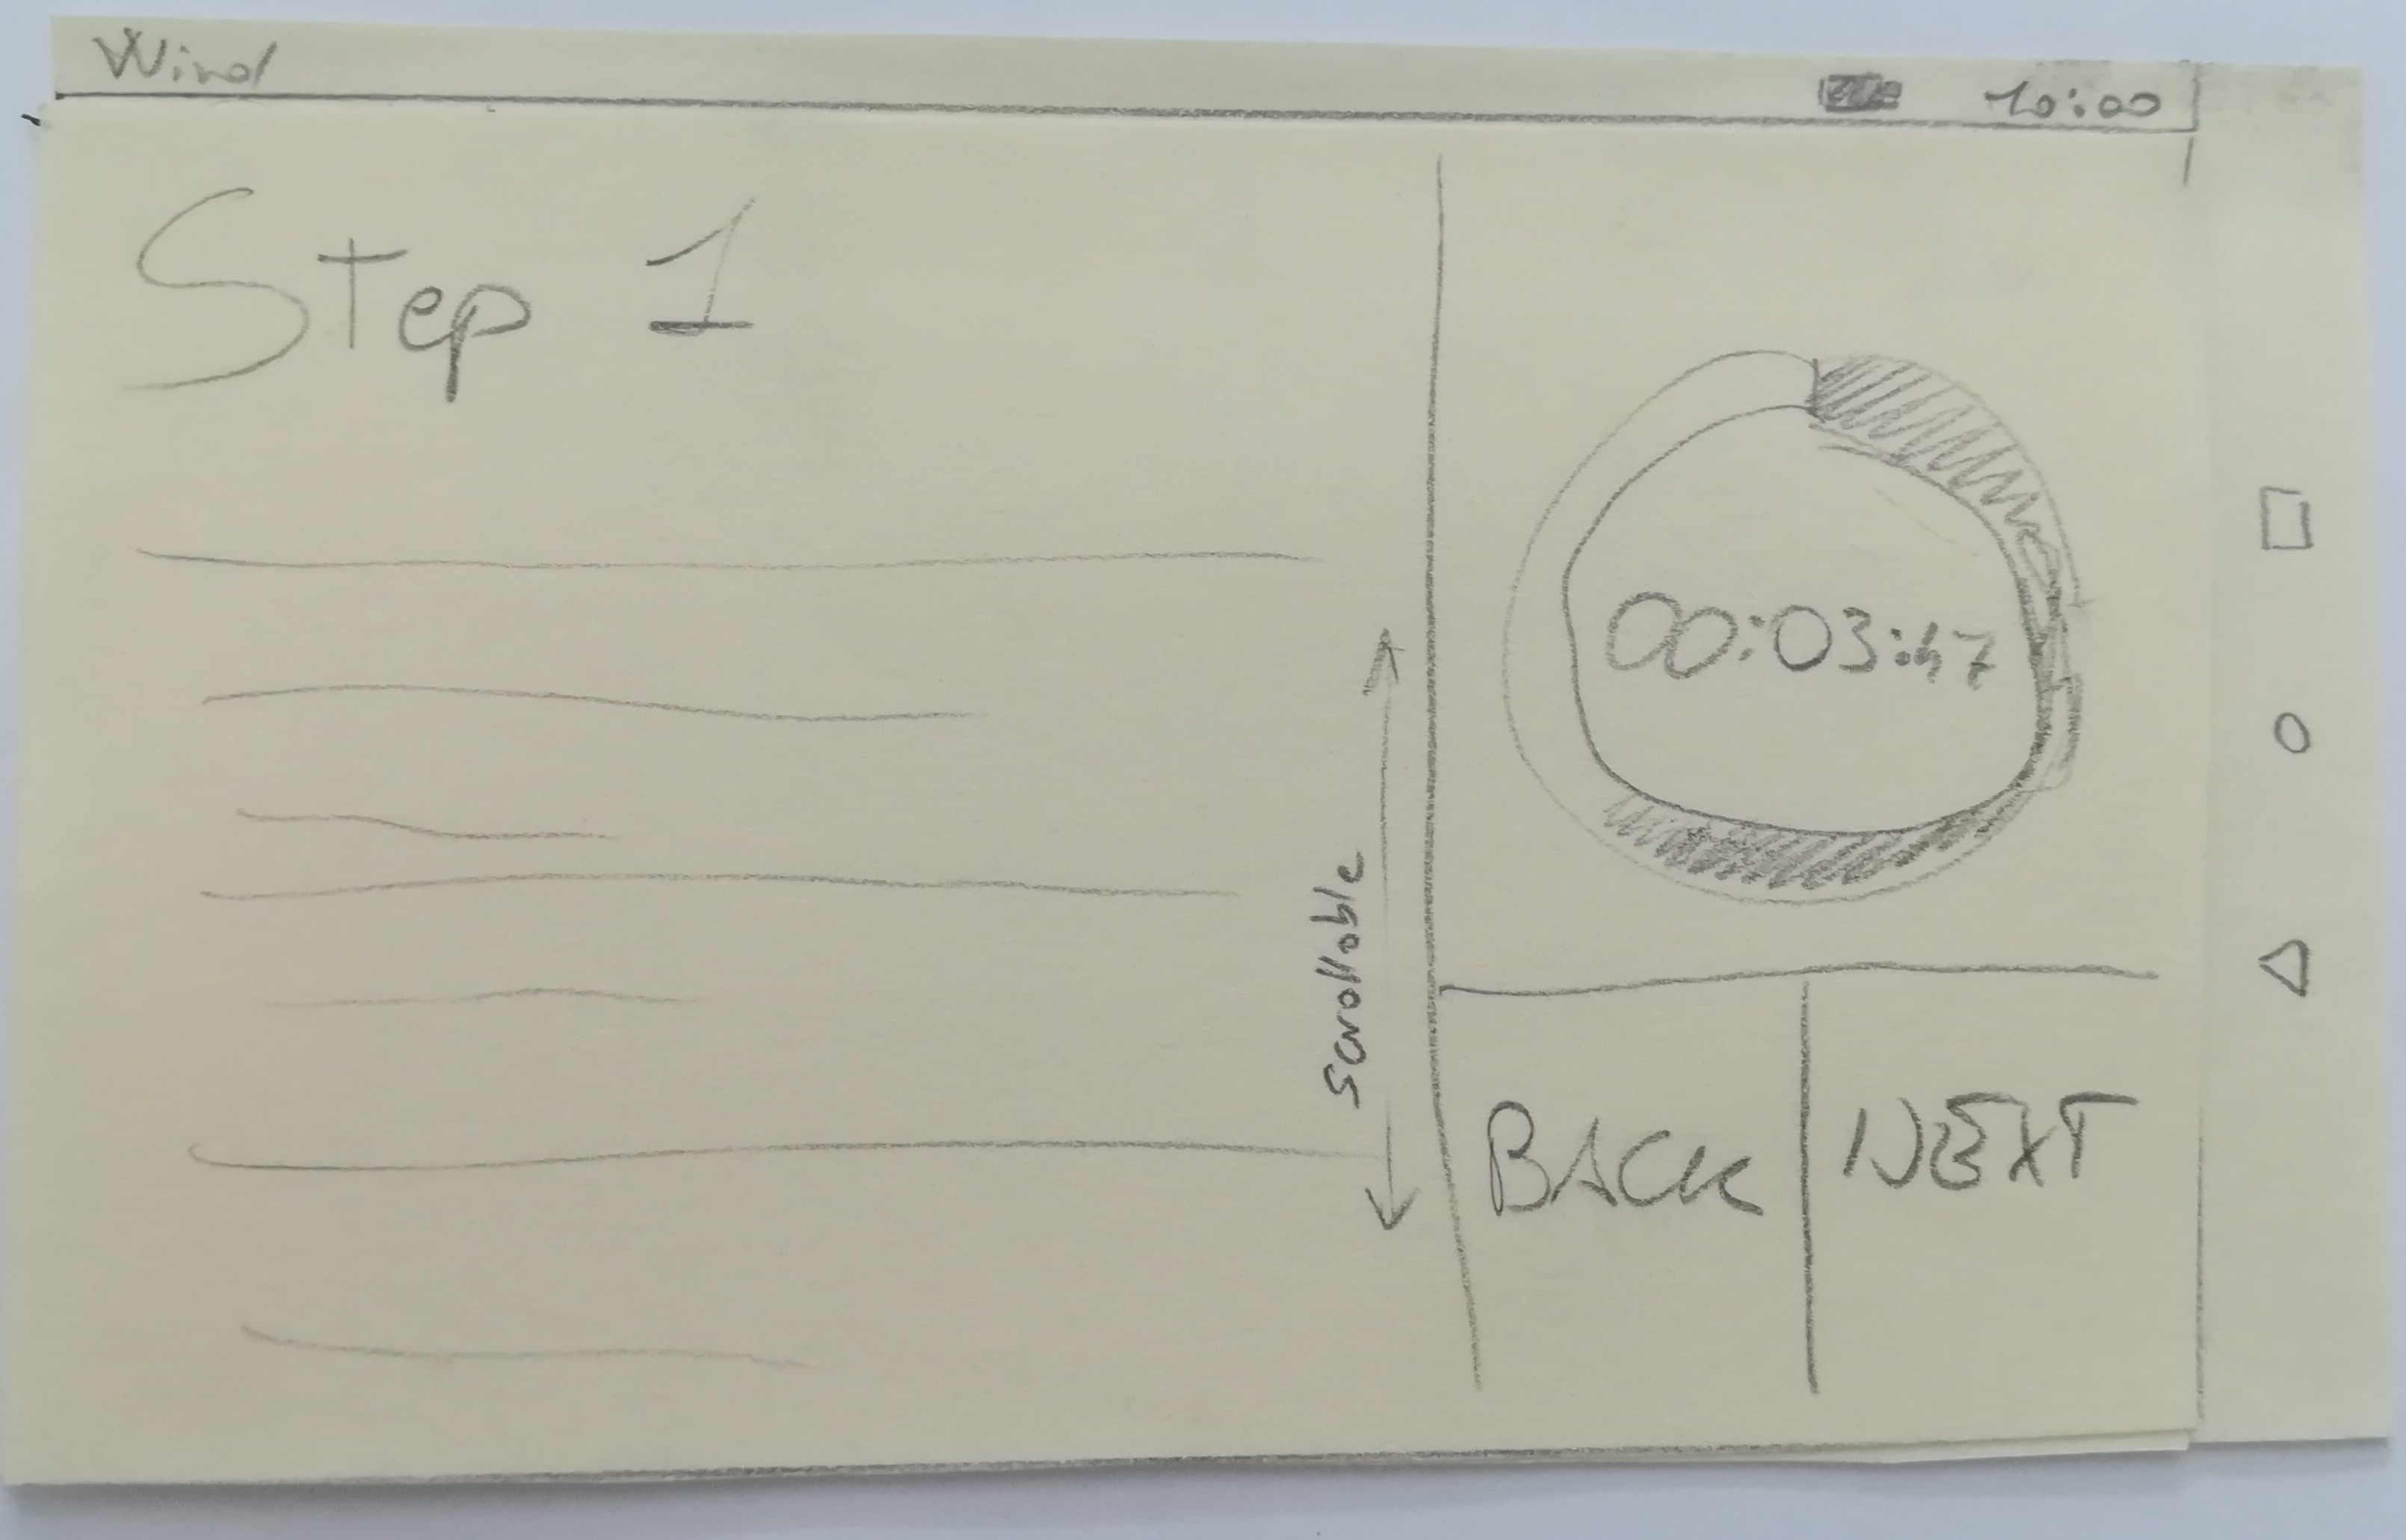
\includegraphics[width=0.78\textwidth]{prototipo1/cuciamo_c}
    \caption{Prime versioni della schermata dell'assistente}
    \label{fig:p1_cuciniamo}
  \end{center}
\end{figure}

\clearpage
In figura \ref{fig:p1_overview} sono mostrate tre versioni differenti della schermata dell'assistente.

\begin{figure}[h]
  \begin{center}
    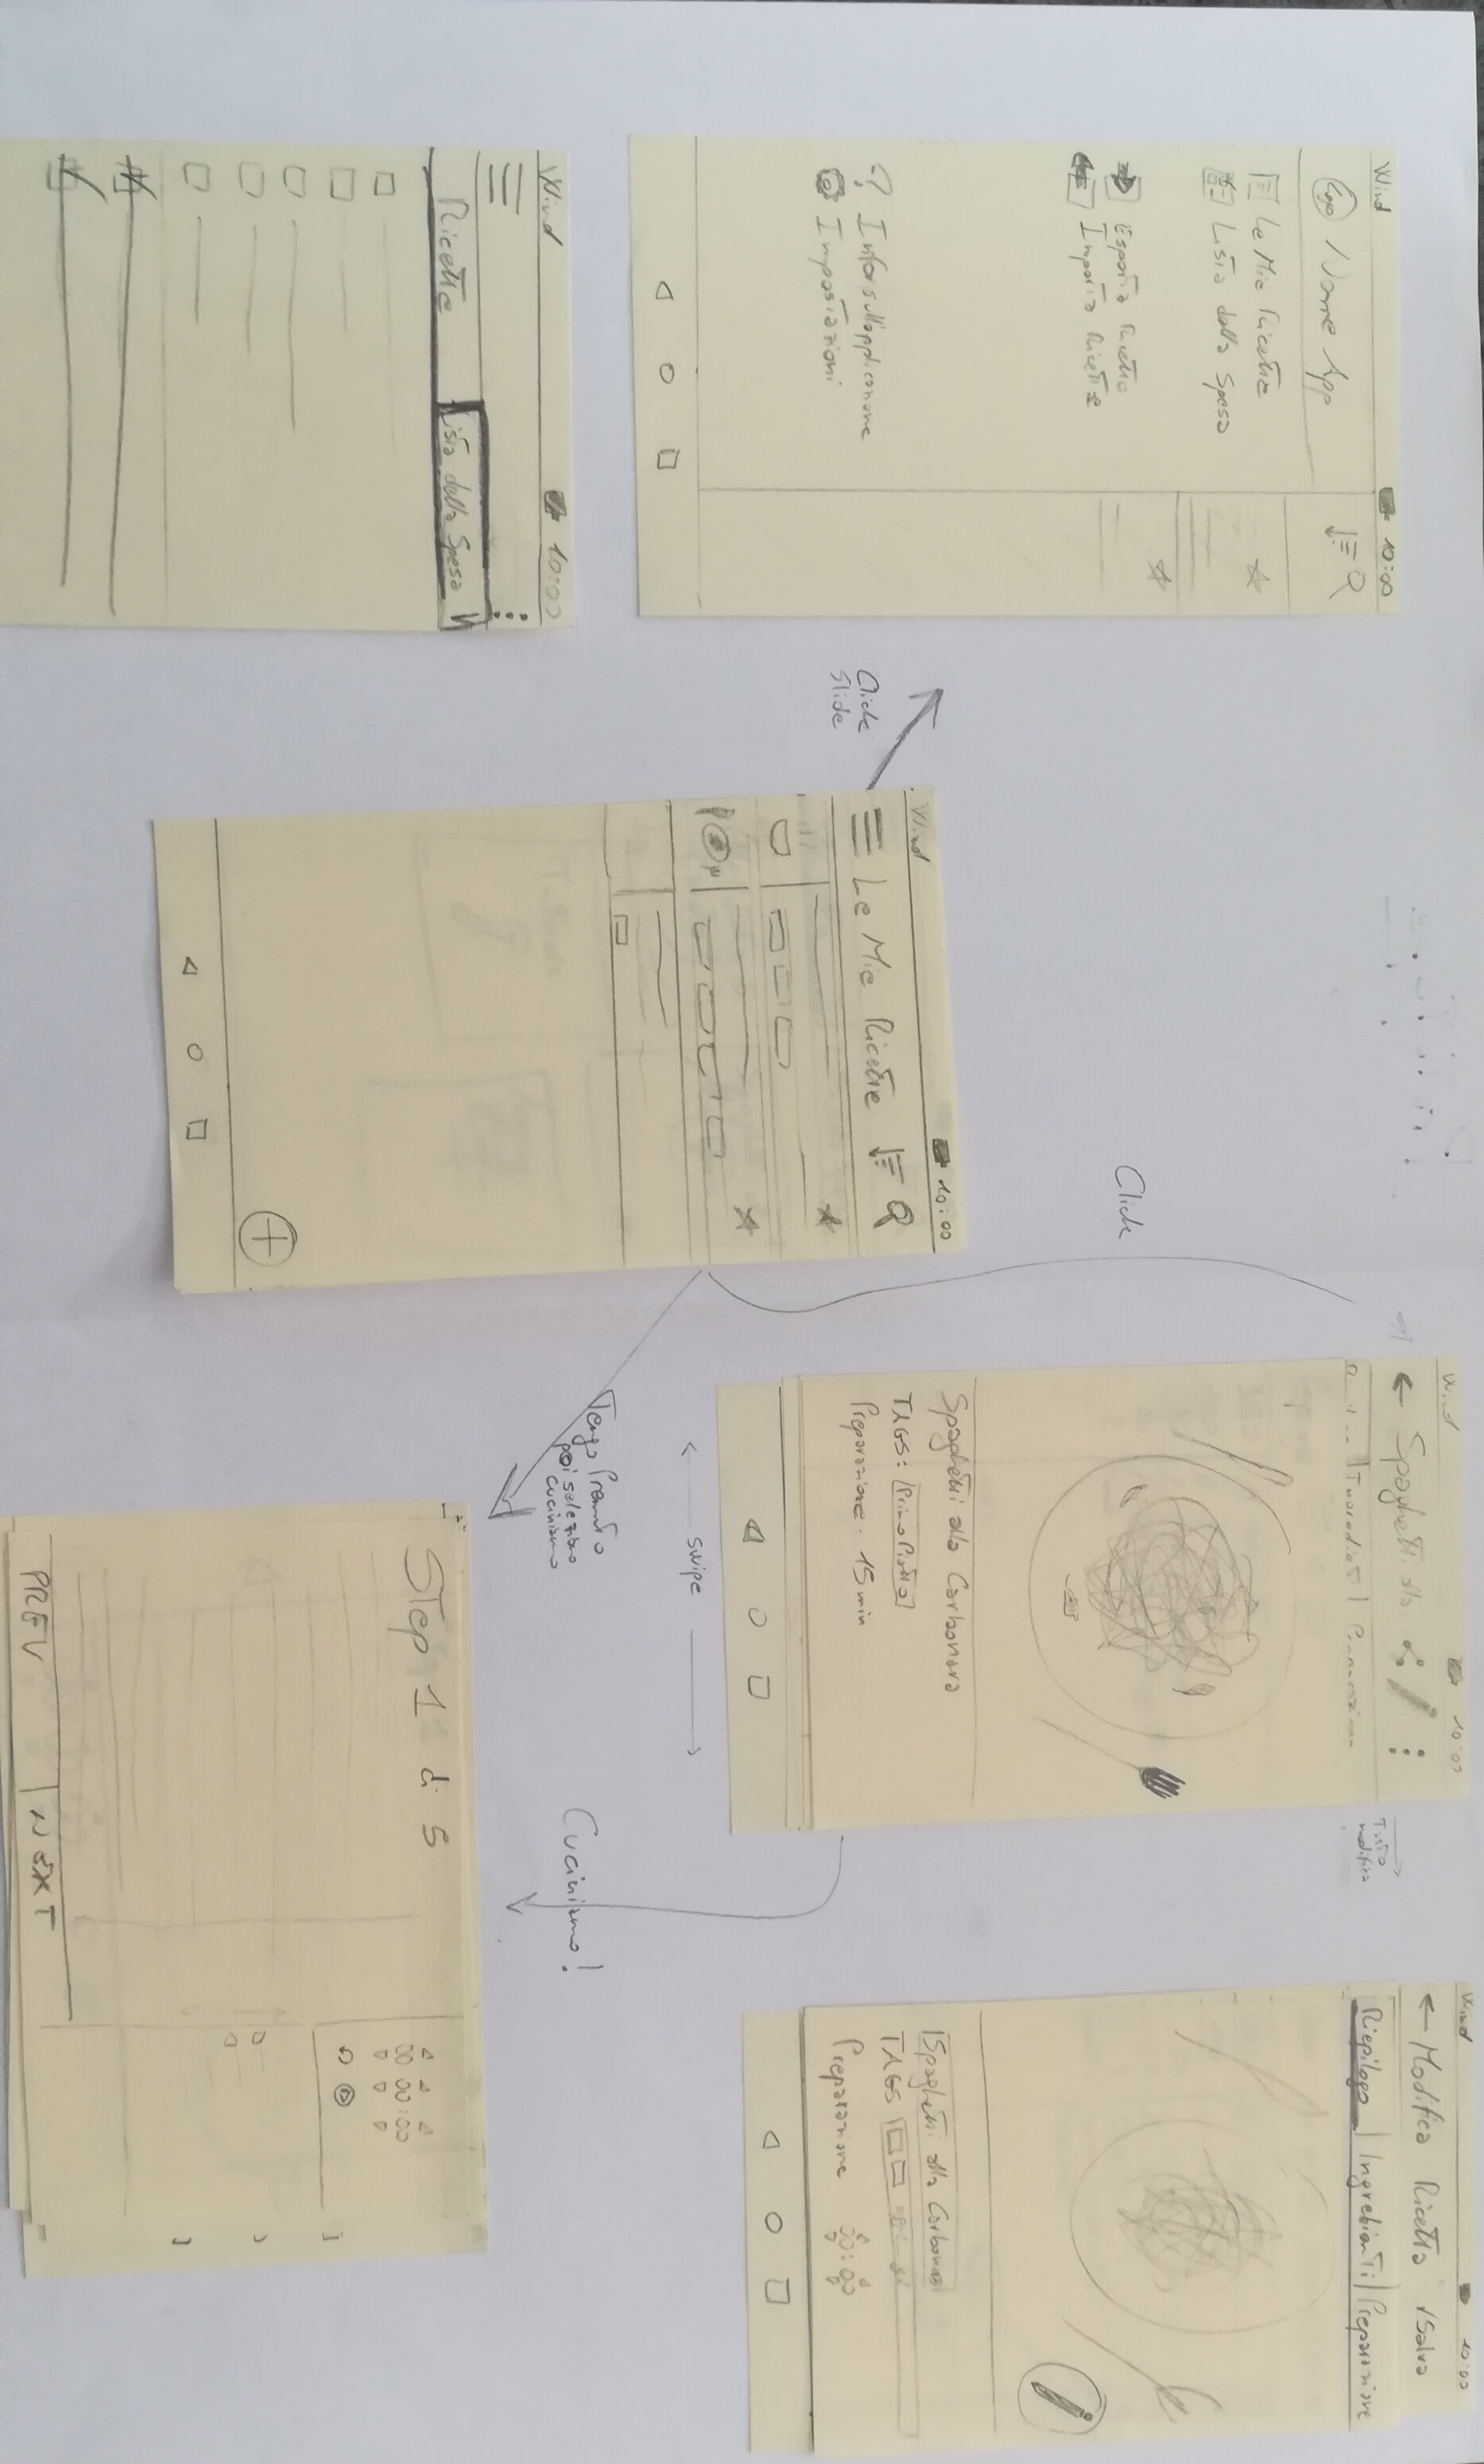
\includegraphics[width=1\textwidth]{prototipo1/overview}
    \caption{Rappresentazione globale delle schermate}
    \label{fig:p1_overview}
  \end{center}
\end{figure}



\clearpage
\subsubsection{Descrizione del Design}
\subsubsection{Valutazione}

\subsection{Secondo Prototipo Low-Fidelity}
\subsubsection{Descrizione del Design}
\subsubsection{Valutazione}

\subsubsection{Design Alternativi}

\subsection{Conclusioni e Design Finale}
